\documentclass[oneside,final,12pt]{extreport}

%% my command
%%%%%%%%%%%%%%
% Путь к файлу с изображениями
\newcommand{\picPath}{images}
% Величина отступа
\newcommand{\indentSpace}{1.25cm}
% Сокращения
\newcommand{\urlTitle}{ $-$ URL: }
%%%%%%%%%%%%%%%


% Изменяем шрифт
\usepackage{fontspec}
\setmainfont{Times New Roman}
\listfiles

% Полуторный интервал
\linespread{1.6}

% Отступ
\setlength\parindent{\indentSpace}

% Математика
\usepackage{mathtools}


% Картинки
\usepackage{graphicx}
\usepackage{subcaption}

% Языковой пакет
\usepackage[russianb]{babel}

% Таблицы
\usepackage{tabularx}

% Настройка подписей к фигурам
% Меняем заголовки картинок
\usepackage[ labelsep= endash]{caption}
\captionsetup{%
   figurename= Рисунок,
   tablename= Таблица,
   justification= centering, singlelinecheck=false
}         

\captionsetup[table]
{
justification= raggedright, singlelinecheck=false
}
% Кирилица в подфигурах
\renewcommand{\thesubfigure}{\asbuk{subfigure}}
% разделитель в подфигурах - правая скобка
\DeclareCaptionLabelSeparator{r_paranthesis}{)\quad }
\captionsetup[subfigure]{labelformat=simple, labelsep=r_paranthesis}

% Добавляем итератор \asbuk,
% чтобы использовать кирилицу
% как маркеры
\usepackage{enumitem}
\makeatletter
\AddEnumerateCounter{\asbuk}{\russian@alph}{щ}
\makeatother

% Меняем маркеры в перечислениях
% Списки уровня 1
\setlist[enumerate,1]{label=\arabic*),ref=\arabic*}
% Списки уровня 2
\setlist[enumerate,2]{label=\asbuk*),ref=\asbuk*}
% Перечисления
\setlist[itemize,1]{label=$-$}
% Удаляем отступы перед и после
% списка
\setlist[itemize]{noitemsep, topsep=0pt}
\setlist[enumerate]{noitemsep, topsep=0pt}

% Красная строка в начале главы
\usepackage{indentfirst}

% Убиваем перенос
\usepackage[none]{hyphenat}

% Перенос длинных ссылок
\usepackage[hyphens]{url}
\urlstyle{same}

% Выравнивание по ширине
\usepackage{microtype}

%\usepackage[fontfamily=courier]{fancyvrb}
%\usepackage{verbatim}%     configurable verbatim
% \makeatletter
%  \def\verbatim@font{\normalfont\sffamily% select the font
%                     \let\do\do@noligs
%                     \verbatim@nolig@list}
%\makeatother

% Границы
\usepackage{vmargin}
\setpapersize{A4}
% отступы
%\setmarginsrb 
%{3cm} % левый
%{2cm} % верхний
%{1cm} % Правый
%{2cm} % Нижний
%{0pt}{0mm} % Высота - отступ верхнего колонтитула
%{0pt}{0mm} % Высота - отступ нижнего  колонтитула

\setlength\hoffset{0cm}
\setlength\voffset{0cm}
\usepackage[top=2cm, bottom=2cm, left=3cm, right=2cm,
]{geometry}
 		
% Настройка заглавиий
\addto\captionsrussian{% Replace "english" with the language you use
  \renewcommand{\contentsname}% содержания
    {\hfill\bfseries
    СОДЕРЖАНИЕ
	\hfill    
    }%
   \renewcommand{\bibname}% списка источников
    {\hfill\bfseries
    	СПИСОК ИСПОЛЬЗОВАННЫХ ИСТОЧНИКОВ
	\hfill
	}% 
}%\

%\renewcommand{\contentsname}{\hfill\bfseries СОДЕРЖАНИЕ \hfill} 

% Настройка  заглавий в главах
\usepackage{titlesec}


%\titleformat
%{\chapter} % command
%[display]
%{
%\bfseries
%} % format
%{
%\thechapter.
%} 	% label
%{ 
%	0 pt
%} % sep
%{    
%\centering
%} % before-code

\titleformat{\chapter}
			[block]
            {\bfseries }
            {\hspace{\indentSpace}\thechapter}
            {1em}
            {\vspace{0mm} }
            [\vspace{14pt}]% Отступ после
% Начальный сдвиг заголовка 50 pt = 1.763888888cm.
% Второй параметр- сдвиг до = 2cm - 50pt
\titlespacing{\chapter}{0pt}
{-0.2361cm}{0pt}

\titleformat{\section}[block]
{\bfseries}{\hspace{\indentSpace}\thesection}{1em}{}

%\titlespacing{\section}{0pt}{0pt}{0pt}

\titleformat{\subsection}[block]
{\bfseries}{\hspace{\indentSpace}\thesubsection}{1em}{}

%\titlespacing{\subsection}{0pt}{0pt}{0pt}

%\titleformat{\section}
%            {\bfseries}
%            {\thechapter.\hspace{1em}}
%            {0pt}
%            {\centering
%            \vspace{0mm} }
%            [\vspace{14pt}]% Отступ после
%\titlespacing{\section}{0pt}{-50pt}{0pt}

% Конец настройка заглавий

% Форматирование списка источников
% Bibl label
\makeatletter
\renewcommand*{\@biblabel}[1]{\indent#1}
\makeatother

% Убрать отсупы в списке источников
\usepackage{lipsum}

% ADD THE FOLLOWING COUPLE LINES INTO YOUR PREAMBLE
%\let\OLDthebibliography\thebibliography
%\renewcommand\thebibliography[1]{
% \OLDthebibliography{#1}
%  \setlength{\parskip}{0pt}
%  \setlength{\itemsep}{0pt plus 0.3ex}
%}

% Change indent
\usepackage{etoolbox}
\patchcmd{\thebibliography}
  {\advance\leftmargin\labelsep}
  {\leftmargin=0pt\itemindent=\labelwidth\advance\itemindent\labelsep}
  {}{}
  
% Define separations
\patchcmd{\thebibliography}{\sloppy}{\itemsep -0.28cm \parsep 0pt \sloppy}{}{}
  



% Добавить точки в оглавление
\usepackage{tocstyle}
\newcommand{\autodot}{}


% Чтобы картинки вставляись
% куда надо
\usepackage{float}

% Для вычисления кол-ва страниц
\usepackage{lastpage}

% Для вычисления кол-ва рисунков и таблиц
%%%
\usepackage{etoolbox}

\newcounter{totfigures}
\newcounter{tottables}

\providecommand\totfig{} 
\providecommand\tottab{}

\makeatletter
\AtEndDocument{%
  \addtocounter{totfigures}{\value{figure}}%
  \addtocounter{tottables}{\value{table}}%
  \immediate\write\@mainaux{%
    \string\gdef\string\totfig{\number\value{totfigures}}%
    \string\gdef\string\tottab{\number\value{tottables}}%
  }%
}
\makeatother

\pretocmd{\chapter}{\addtocounter{totfigures}{\value{figure}}\setcounter{figure}{0}}{}{}
\pretocmd{\chapter}{\addtocounter{tottables}{\value{table}}\setcounter{table}{0}}{}{}
%%%

% Режим релиза
\sloppy
\usepackage{layout}

%\renewcommand{\arraystretch}{1.6}

\newcommand{\cmmnt}[1]{\ignorespaces}
\newcommand{\bs}{\boldsymbol}
\usepackage{breqn}

% Change intemize intend
\usepackage{calc}

\usepackage{listings}

\newlength{\mylength}
\settowidth{\mylength}{$-$\textvisiblespace}

\setlist{itemindent= \mylength + \indentSpace ,leftmargin=0pt}
\begin{document}
\tableofcontents
\newpage
\textbf{Введение}
\addcontentsline{toc}{chapter}{Введение}

Машинное обучение в современном мире ставит перед собой довольно амбициозные задачи: мы пытаемся научить машину понимать человеческую речь, видеть картинки и ориентироваться в пространстве, понимать какие-то сложные человеческие концепции и так далее. Все это требует извлечения очень сложных зависимостей из оригинальных данных,  и соответственно, чтобы извлекать эти сложные зависимости, нам требуются сложные модели.

Наиболее сложной и продвинутой моделью машинного обучения  на текущий момент является нейронная сеть — про нее и будет идти речь в данной курсовой работе.  На текущий момент существуют очень большие нейронные сети, которые могут делать потрясающие вещи.  Например, существует сеть GPT-3, и в ней ученые смогли обучить 175 миллиардов параметров. Просто ради интереса можно привести числа о том, сколько нейронов находится в голове человека. Ученые говорят, что где-то от 20 до 80 миллиардов, то есть формально говоря, в нейронной сети GPT-3 нейронов больше, чем в голове человека, и при этом она действительно может делать довольно интересные вещи. 

Однако у такого подхода есть и обратная сторона медали — эти модели получаются очень трудно используемыми: они получаются тяжело обучаемыми, они занимают очень много места, а также они очень долго считают свой ответ.

В целом, если мы говорим про какую-то исследовательскую работу, тогда это небольшая проблема: там действительно мы ставим перед собой задачу просто получить самую лучшую модель по качеству. Однако, если мы с вами возвращаемся в реальный мир, то ситуация немного меняется. 

Реальные примеры использования машинного обучения требуют более жестких требований к самим алгоритмам. Хочется одновременно получать и хорошее качество результатов, и высокую скорость обработки; при этом было бы неплохо, если бы наша модель была автономной, а также ресурсоэффективной. 

Примеров таких задач огромное количество. Например, это улучшение фотографий в наших телефонах — сделали какую-то фотографию, и она сразу стала более лучшего качества. Это возможно, потому что она была сразу обработана алгоритмом. Также можно привести автоматический перевод текстов с картинки, голосовые ассистенты, которые работают в каждом телефоне, и вплоть до беспилотных автомобилей. Все эти алгоритмы должны работать быстро, качественно и, желательно, не требовать дополнительного взаимодействия с сетью Интернет.

Отметим, что такое вообще мобильные девайсы или мобильные устройства. Самые очевидные представители мобильных устройств — это, конечно же, телефоны и смартфоны. По состоянию на 2021 год насчитывают более 14 миллиардов телефонов и смартфонов по всему миру, то есть немного больше, чем количество людей на планете. 
Однако стоит отметить, что телефоны и смартфоны — это не единственные представители мобильных устройств. Также существует гигантское количество различных приборов, аудиосистем, роутеров, умных вещей, часов и так далее. То есть много каких-то маленьких устройств, которые при этом имеют процессор и умеют вычислять и решать какие-то несложные в плане ресурсов задачи.
 
Все эти приборы можно было бы каким-то образом улучшить, если бы мы могли добавить к ним элементы алгоритмов искусственного интеллекта, чтобы они могли лучше выполнять поставленную перед ними задачу. Однако, возникает проблема с тем, что у них очень жесткие требования к алгоритмам, которые мы можем на них запускать. 

К таким требованиям относится то, что они должны работать в рамках очень ограниченной памяти, они должны использовать ограниченное число тактов процессора, потому что процессор на самих устройствах довольно слабый, желательно, чтобы они по минимуму использовали или не использовали вовсе интернет-соединение, так как на некоторых девайсах его просто нет, а на некоторых это очень дорого, и, что немаловажно, у всех таких девайсов чаще всего очень ограничено количество батареи, которую они могут использовать для своей работы, и поэтому никто бы не хотел разряжать устройство алгоритмом слишком быстро. 
 
Можно пытаться решить эту задачу таким классическим образом: мы берем большие модели с огромным количеством параметров и запускаем их на гигантских кластерах. В итоге все приложения пользователей будут просто общаться с этими серверами и получать нужную информацию от них. Однако, модели все еще остались достаточно большими, и даже на таких больших мощностях они могут работать медленно, мы можем тратить на их поддержание огромное количество денег, и при этом не стоит забывать, что нам все еще требуется интернет-соединение для каждой работы нашего алгоритма. 

Если же идти другим путем и пытаться запускать эти модели на самих устройствах, возникает другая проблема: устройства очень слабые, и им просто может не хватить ресурсов, чтобы запустить эти модели; или даже если мы все-таки смогли их запустить, они могут работать слишком медленно или моментально расходовать всю батарею, которая есть на устройстве. Таким образом, если мы говорим про то, чтобы запускать реальные модели машинного обучения в каких-то практических случаях, тогда мы должны подумать о том, как бы нам оптимизировать размер этой модели и скорость ее выполнения.
 
В этой курсовой работе будут разобраны эффективные методы вычислений корневых операций в нейронных сетях, какие модели машинного обучения можно оптимизировать и каким образом, какие различные архитектуры подходят для запуска на мобильных устройствах. Особое внимание будет уделено таким процессам оптимизации, как квантизация и прунинг. Будут рассмотрены существующие фреймворки для этих инструментов, в частности NNCF, почему именно этот фреймворк подходит для промышленого машинного обучения и зачем нам в целом иметь какой-либо фреймворк для алгоритмов сжатия моделей.

В практической части представлена реализация алгоритмов дистилляции знаний между нейронными сетями, статический прунинг после тренировки, итеративный прунинг, методы квантизации после тренировки и динамический вид квантизации во время тренировки. Для проверки этих алгоритмов были взяты сверточные и полносвязанные нейронные сети, в частности для алгоритмов сжатия была выбрана наиболее популярная архитектура ResNet и академический датасет FashionMNIST. В заключительной части мы посмотрим и применим фреймворк NNCF к реальной задаче антиспуфинга лиц, где в качестве основы нейронной сети взята MobileNetV3.

\chapter{Структурная оптимизация нейронных сетей}
Структурная оптимизация может включать в себя три части: оптимизация алгоритмов производимых вычислений, поиск архитектурных решений и дистилляция знаний. 

Сегодня, занимаясь разработкой исскуственных нейронных сетей все исследователи в той или иной мере используют уже готовые фреймовроки, такие как Tensorflow, Pytorch, Theano. Они позволяют не задумываться о тонкостях реализации таких операций как матричные вычисления, операции свертки, взятие градиента и так далее, а сосредоточиться на основном алгоритме для решения поставленной задачи. Однако, важно понимать, что эффективная реализация и оптимизация подобных низкоуровневых компонентов очень важна и правильное использование подобных инструментов позволит ускорить вычисления в разы. 

Например, давайте рассмотрим умножение матриц. Это является ключевой операцией в любом алгоритме исскуственного интелекта, связанного с нейронными сетями. На рисунке 1.1 представлен наивный алгоритм реализации матричного умножения на языке программирования С

\begin{figure}
\begin{center}
  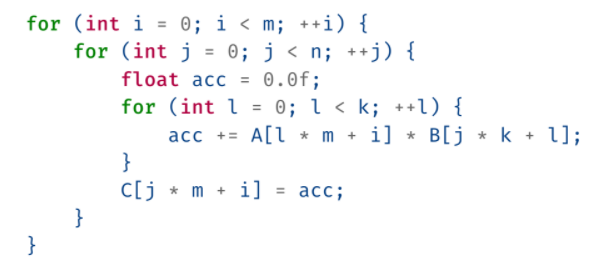
\includegraphics{\picPath/structure_1.png}
  \caption{Код реализации матричного умножения на языке С}
  \label{fig:structure_1}
  \end{center}
\end{figure}

Что не так с этим алгоритмом? Очевидно, что временая сложность такого алгоритма будет порядка $O(n^3)$ для квадратных матриц. Поэтому нужно попытаться как-то оптимизировать данный алгоритм. 

Существует такая программа для вычислений матриц, как GEMM (General matrix multiplication). Она предоставляет  интрефейс для вычислений матриц подобного вида: $a*AB + b*C$. Это одна из трех программ коплекса вычислений линейной алгебры BLAS (Basic Linear Algebra Subprograms). BLAS включает в себя стандартизированный интерфейс для работы с объектами линейной алгебры, а именно включает в себя 3 уровня подпрограмм:

\begin{itemize}
\item векторные вычисления
\item матрица-вектор
\item матрица-матрица
\end{itemize}

Множество современных библиотек исаользуют реализацию GEMM с множеством дополнительных оптимизаций под разные архитектуры железа. 

Рассмотрим как представлена x86,64 архитектура центрального процессора. На рисунке 1.2 представлена пирамида иерархии памяти для процессора, справа изображен пример как распределена кэш-память для процессора Intel core i7.

Что же ограничивает производительность нашего алгоритма? Здесь может быть две причины. Первая это то, что у нашего процессора ограничено количество операций в секунду, которое мы не можем превзойти. Но есть другой вариант, когда наш алгоритм сильно завязан на перессылке данных из оперативной паяти в процессор и это тоже может очень сильно ограничивать его скорость. В уравнении (1.1) представлена оценка производительности алгоритма в термине FLOPS (FLoating-point Operations Per Second) 
\begin{figure}[H]
  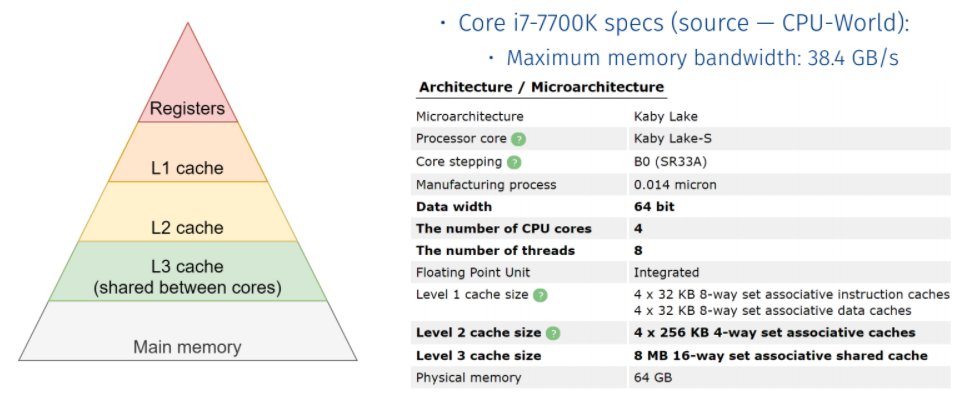
\includegraphics[width=\linewidth]{\picPath/structure_2.png}
  \caption{Иерархия памяти на примере процессора Intel Core I7. Помимо основной памяти, можно выделить три уровная кэша, наверху расположен регистер процессора, образующий сверхбыструю оперативную память}
  \label{fig:structure_2}
\end{figure} 

\begin{equation}
FLOPS \leq min( peak\ FLOPS,\ \frac{FLOP}{bytes} * peak\ bindwidth),
\end{equation}

где $peak\ bandwidth$ – пропускная способность памяти,

$\frac{FLOP}{bytes}$ – интенсивность вычислений

Получается так называемая Roofline model, на рисунке 1.3 представлено изображение, показывающее зависимость интенсивности вычислений от производительности реализации алгоритма. Эффективной реализацией алгоритма (эффективной оптимизацией под аппаратуру) считается та реализация, у которой производительность близко находится к прямым ограничения по памяти и по количеству операций в секунду конкретного процессора. Ключевой фактор любого алгоритма – это его интенсивность вычисления.
\begin{figure}[H]
\begin{center}
  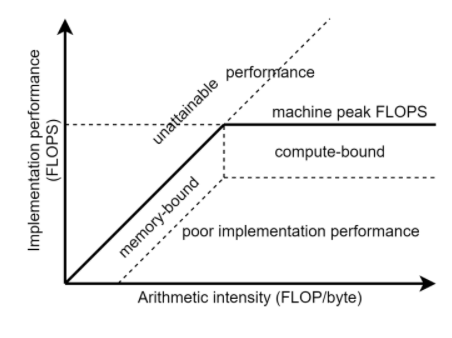
\includegraphics{\picPath/structure_4.png}
  \caption{Roofline model}
  \label{fig:structure_4}
 \end{center}
\end{figure}

При наивной реализации матричного произведения не эффективно используется память и происходит многократная перессылка данных в оперативной памяти и данный алгоритм будет иметь низкую интенсивность вычислений, примерно $\frac{1}{2}$.

Первый подход к оптимизации использования кэш памяти в данном алгоритме  это так называемый блокинг. На рисунке 1.4 представлена визуализация данного процесса.

\begin{figure}[H]
\begin{center}
  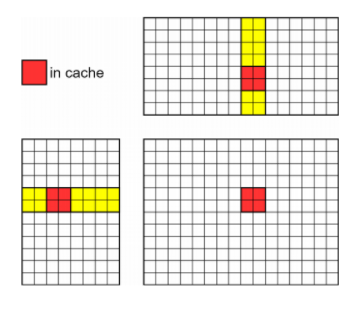
\includegraphics{\picPath/structure_5.png}
  \caption{Визуализация операции блокинга}
  \label{fig:structure_5}
  \end{center}
\end{figure}

Мы разбиваем матрицы на небольшие блоки размером bxb и мы можем применить матричное произведение для этих блоков, как показано в уравнении (1.2):
\begin{equation}
C_{pq}=\sum_{r=1}^{k/b}A_{pr}B_{rq}\ \ \ \ \ \
p=1,...,\frac{m}{b};\ \
q=1,...,\frac{n}{b}
\end{equation}

Мы также будем использовать тройной цикл, но интенсивность вычислений будет выше. У нас будет всего $\frac{mnk}{b^3}$ внутренних итераций (для матриц размером $m \times n$ и $n \times k$). Теперь на каждой итерации считывается $2b^2$ элементов, а количество операций в секунду  для вычисления блока матрицы $С – 2b^3$, поэтому итоговая интенсивность вычислений будет следующая, как показано в уравнении (1.3)
\begin{equation}
    \frac{2mnk}{(\frac{mnk}{b^3} \cdot 2b^2 \cdot sizeof(float))} = \frac{b}{4}
\end{equation}

Параметр b выбирается настолько большим, насколько нам позволяет вместить кэш. В данном примере мы считали, что у нас всего один кэш, однако как было уже сказано выше, в процессорах несколько кэшей разного уровня. Поэтому для дальнейшего ускорения мы можем сделать блокинг на нескольких уровнях кэша и даже на уровне регистров. Есть также подходы по переупорядочению элементов, чтобы элементы блоков лежали рядом, при этом выборка будет из соседних участков памяти и это еще сильнее должно ускорить алгоритм. Далее у многопоточных процессоров есть векторные инструкции  для векторизации вычислений в циклах.
Все это способствуют ускорению и оптимизации вычислений в наших алгоритмах во много раз.

\section{Эффективная реализация свертки}
Операция свертки – это ключевая операция для сверточных нейронных сетей. Поэтому ее оптимизация очень важна для производительной работы алгоритма. Наивная реализация этой операции может быть представлена в виде скользящего окна размером $k \times k$ и для каждого положения этого окна мы будем производить операции поэлементного умножения и последующей суммы. Однако это опять неэффективное использование памяти и многократная перессылка данных из оперативной памяти и обратно, что ведет к низкой интенсивности вычислений. Чтобы ускорить этот алгоритм мы можем выразить операцию свертки через матричные операции. Такое преобразование называется image to column. 

Рассмотрим свертку одного одноканального изображения размером $4 \times 4$ пикселя (значения пикселей обозначены через $X$). Сворачивать будем с ядром из одного фильтра размером $3 \times 3$, веса обозначены через $W$. Для простоты примем $stride = 1$. Тогда выход $Y$ будет иметь размерность $1 \times 1 \times 2 \times 2$ (в данном случае на входе одно изображение - это первая единица в размерности, в ядре один фильтр - это вторая единица в размерности выхода). На рисунке 1.5 представлена визуализация операции свертки в простейшем виде.
\begin{figure}[H]
\begin{center}
  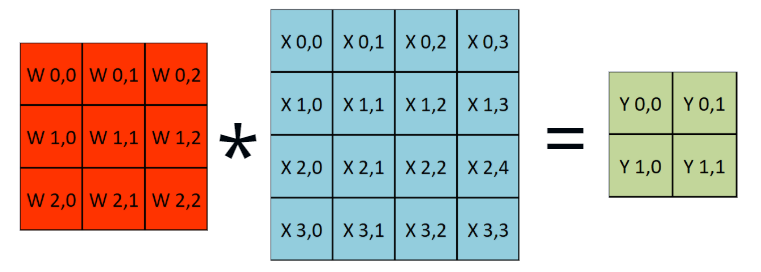
\includegraphics[width=\linewidth]{\picPath/svertra_1.png}
  \caption{ визуализация операции свертки}
  \label{fig:svertra_1}
  \end{center}
\end{figure}
Оказывается выход свертки можно получить умножением матриц, как показано на рисунке 1.6. 
\begin{figure}[H]
\begin{center}
  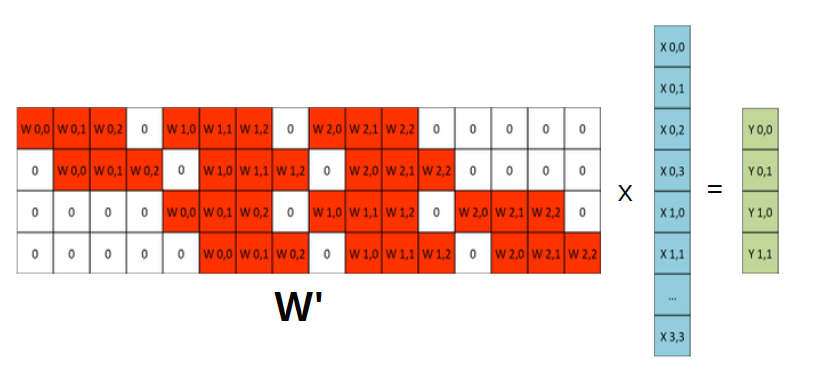
\includegraphics[width=\linewidth]{\picPath/svertra_2.png}
  \caption{Image2column.Представление операции свертки матричным произведением}
  \label{fig:svertra_2}
  \end{center}
\end{figure}
Давайте перейдем от простого случая к общему:
\begin{itemize}
\item Если фильтров в ядре больше одного. Заметим, что для каждого фильтра, матрица $W’$ будет умножаться на один и тот же вектор изображения. Значит, можно сконкатенировать матрицы фильтров ядра по вертикали и за одно умножение получить ответ для всех фильтров.
\item Если на входе более одного изображения: заметим, что матрица $W’$ одинакова для всех изображений батча, то есть, можно каждое изображение вначале вытянуть в столбец, а затем эти столбцы для всех изображений батча сконкатенировать по горизонтали.
\item Если в изображении больше одного слоя, вначале выполним преобразования входа и ядра для каждого слоя, а затем сконкатенируем: вектора разных слоев входа в один большой вектор, а матрицы ядра соответственно в одну длинную матрицу. И мы получим сложение от выходов по слоям в процессе перемножения матриц.
\end{itemize}

На рисунке 1.7 представлена визуализация подхода Image2Column для много-канального изображения. То есть даже в самом общем случае мы за одно умножение матриц можем получить ответ.

В реализации данной операции есть один недостаток. Полученная матрица ядер является разреженной и содержит много нулей, это снижает эффективность метода.

Давайте получим тоже самое, при этом уберем этот недостаток. Пусть в этот раз на входе батч из одного трехслойного (RGB) изображения размером $3 \times 3$. Пусть ядро имеет 2 фильтра шириной и высотой 2 пикселя. Тогда выход должен иметь размерность $1 \times 2 \times 2 \times 2$. Пусть $W$ - веса ядра, $X$ - значения входной матрицы, $Y$ - значения на выходе. Для простоты слои изображения и слои фильтров ядра покрашены в цвета. На рисунке 1.8 представлена визуализация операции свертки для двух фильтров и RGB изображения

\begin{figure}[H]
\begin{center}
  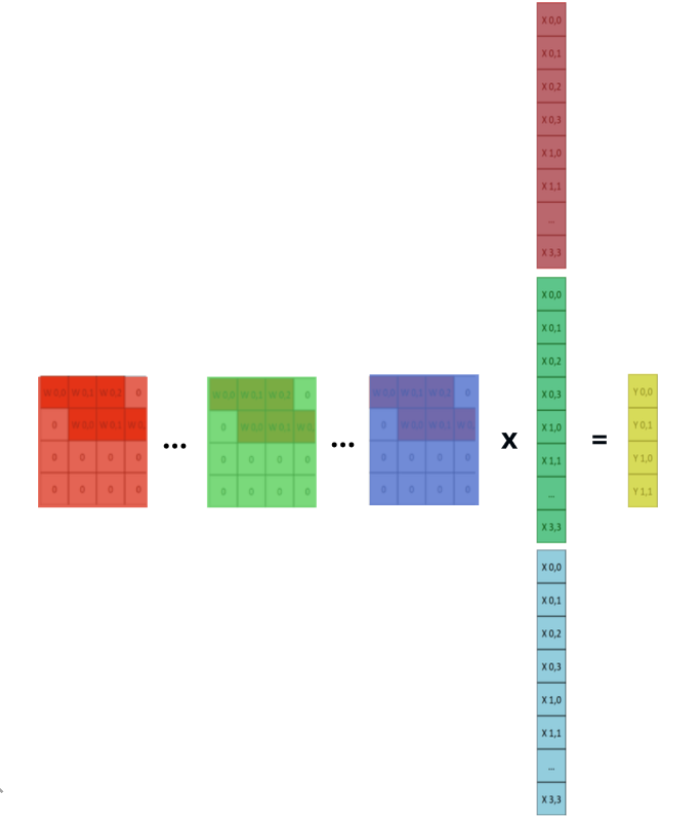
\includegraphics[width=\linewidth]{\picPath/svertra_3.png}
  \caption{многоканальный Image2Column}
  \label{fig:svertra_3}
  \end{center}
\end{figure}

\begin{figure}[H]
\begin{center}
  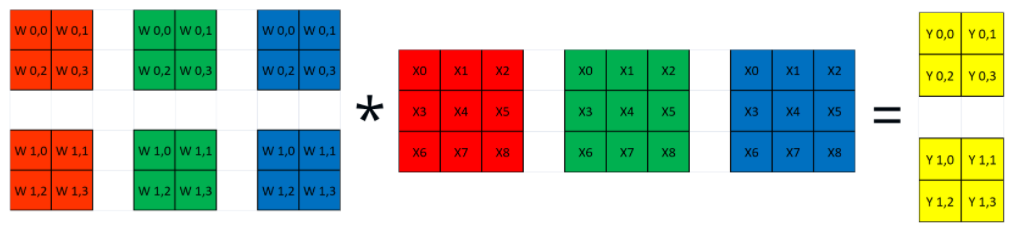
\includegraphics[width=\linewidth]{\picPath/svertra_4.png}
  \caption{Визуализация операции свертки для двух фильтров и трех каналов изображения}
  \label{fig:svertra_4}
  \end{center}
\end{figure}
Если в первом матричном способе мы вытягивали изображения в столбцы, то теперь будем вытягивать фильтры кернела в строки, как показано на изображении 1.9.

Если изображений в батче больше одного: преобразования ядра от этого не меняется, а преобразованные матрицы входных изображений конкатенируются по горизонтали. Теперь, используя GEMM для матричного произведения мы можем добиться высокой оптимизации операции свертки. 

Но с таким подходом есть все же свои проблемы. Когда мы конструируем подобную матрицу в общем случае у нас происходит дублирование данных. Почти каждый элемант дублируется  $k^2$ раз, где $k$ – это размер ядра. Конструируем матрицу в главной, глобальной памяти и занимаем достаточно много ее количества. На практике напрямую такую матрицу в память не сохраняют, а подгружают ее частями. Например, при реализации GEMM для GPU используется разделяемая память, которая достаточно быстрая и используют указатели при хранении объектов для более эффективного использования памяти.

Следующий подход к реализации свертки основан на быстром преобразовании Фурье. Дискретное преобразование Фурье (Discrete Fourier Transform) — это одно из преобразований Фурье, широко применяемых в алгоритмах цифровой обработки сигналов, а также в других областях, связанных с анализом частот в дискретном (к примеру, оцифрованном аналоговом) сигнале. Дискретное преобразование Фурье требует в качестве входа дискретную функцию. Такие функции часто создаются путём дискретизации (выборки значений из непрерывных функций). Дискретные преобразования Фурье помогают решать дифференциальные уравнения в частных производных, его модификации применяются в сжатии звука в MP3, сжатии изображений в JPEG, выполнять такие операции, как свёртки и др. Определение представлено в уравнении (1.4).

\begin{figure}[H]
\begin{center}
  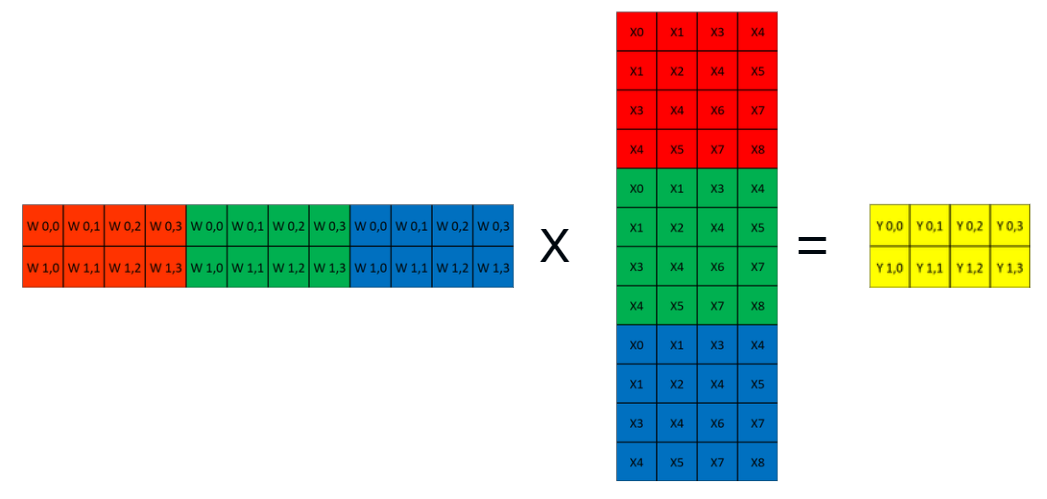
\includegraphics[width=\linewidth]{\picPath/svertra_5.png}
  \caption{Представление операции свертки через матричное произведение более эффективным путем. Избавляемся от разреженных матриц}
  \label{fig:svertra_5}
  \end{center}
\end{figure}


\begin{equation}
X_k = \sum_{n=0}^{N-1}x_n\cdot e^{\frac{-2\pi i}{N}kn}=\sum_{n=0}^{N-1}x_n\cdot[cos(\frac{2\pi}{N}kn)-i\cdot sin(\frac{2\pi}{N}kn))]    
\end{equation}

Это преобразование обратимо и обратная функция имеет вид, как показона в уравнении (1.5):
\begin{equation}
X_k = \frac{1}{N}\sum_{n=0}^{N-1}x_n\cdot e^{\frac{2\pi i}{N}kn}
\end{equation}

Попробуем оценить вычислительную сложноть DFT. 
Наивная оценка данной операции порядка $ О (N^2) $. Однако, если мы разобьем функцию на сумму четных и нечетных индексов (уравнение (1.6))
\begin{equation}
\begin{split}
X_k = \sum_{m=0}^{N/2-1}x_{2m}\cdot e^{\frac{-2\pi i}{N}(2m)k} + \sum_{m=0}^{N/2-1}x_{2m+1}\cdot e^{\frac{-2\pi i}{N}(2m+1)k} = \\ =\sum_{m=0}^{N/2-1}x_{2m}\cdot e^{\frac{-2\pi i}{N/2}(m)k} + e^{\frac{-2\pi i}{N}k}\sum_{m=0}^{N/2-1}x_{2m+1}\cdot e^{\frac{-2\pi i}{N/2}mk}
\end{split}
\end{equation}

Если $k < N/2-1$, то финальная сумма для $k$-ых элементов DFT четных  и нечетных сигналов входа будет соответственно:
\begin{equation}
X_k = E_k + e^{\frac{-2\pi i}{N}}O_k
\end{equation}

Для $k’ = k + N/2$:
\begin{multline}
X_{k+\frac{N}{2}} = \sum_{m=0}^{N/2-1}x_{2m}\cdot e^{\frac{-2\pi i}{N/2}m(k+\frac{N}{2})} + e^{\frac{-2\pi i}{N}(k+N/2)}\sum_{m=0}^{N/2-1}x_{2m+1}\cdot e^{\frac{-2\pi i}{N/2}m(k+\frac{N}{2})} = ...\\  = E_k - e^{\frac{-2\pi i}{N}k}O_k
\end{multline}

Вторая половина выходов тоже выражается через компоненты четных  и нечетных индексов. То есть получили рекурсивную процедуру и если предположить, что N это степень двойки, то мы получим сложность порядка $О(NlogN)$.

Полезное свойство DFT заключается в том, что DFT реального входа (нулевая мнимая часть) это палидром вида:
$$[X_0\ \ X_1\ \ X_2\ \ X_3\ \ X_4\ ... \ X_3\ \ X_2\ \ X_1]$$

Благодаря нулевой фазе и периодичности синусоидальных функций мы можем вычислять и хранить примерно половину всех данных. Доказана теорема свертки (уравнение (1.9)): 
\begin{equation}
\begin{split}
{(f*g)(x)}
\Leftrightarrow 
{(F \cdot G )(\xi)}\\
{(f \cdot g)(x)}
\Leftrightarrow 
{(1/MN)(F*G )(\xi)}
\end{split}
\end{equation}

То есть мы применяем прямое преобразование Фурье для входа и фильтра, покомпонентно перемножаем и затем делаем обратное преобразование. Свертка двух функций в пространственном базисе эквивалентна по элементному произведению в частотном. Тогда как наивный метод посредством скользящего окна требует $MNmn$ операций для свертки изображения размера $M \times N$ с ядром размерности $m \times n$. Свертка же посредством преобразования Фурье, вместе со всеми преобразованиями требует $2MNlog2(MN)$ операций, что в случае большой размерности ядра значительно уменьшает число вычислений.

Еще один способ вычислить эффективно свертку – применить так называемую свертку Винограда. Стандартный подход к вычислению линейной свертки требует 6 операций умножений. Данный алгоритм сокращает количество умножений до 4, при этом увеличив количество сложений вещественных чисел. Но так как умножение это более дорогая операция, то мы можем получить выйгрыш в скорости. в уравнении (1.10) представлена формула для вычисления одномерной свертки таким способом:
\begin{equation}
F(2,3) = \begin{bmatrix}
d_0& d_1 & d_2\\ 
d_1&  d_2& d_3
\end{bmatrix} \cdot \begin{bmatrix}
g_0\\ 
g_1\\ 
g_2
\end{bmatrix} = \begin{bmatrix}
m_1+m_2+m_3\\ 
m_2-m_3-m_4
\end{bmatrix}
\end{equation}
где\ \ $m_1=(d_0-d_2)g_0$\\
$m_2=(d_1+d_2)\frac{g_0+g_1+g_2}{2}$\\
$m_3=(d_2-d_1)\frac{g_0-g_1+g_2}{2}$\\
$m_4=(d_1-d_3)g_2$

В целом можно подвести итог по текущему состоянию в области оптимизации сверточных операций (согласно статьям и исследованиям):
\begin{itemize}
\item DFT эффективен только для больших ядер, что редко встречается в современных моделях глубокого обучения. Поэтому данный метод используется редко.
\item Winograd - это самый прорывной алгоритм для сверток $3 \times 3$, однако он требует очень тщательной оптимизации под конкретное железо из-за низкой вычислительной интенсивности.
\item GEMM по-прежнему является выбором по умолчанию в средах глубокого обучения (и, конечно, он используется на различных несверточных уровнях, таких как self-attention модулях)
\end{itemize}

Подведем итог:
\begin{itemize}
\item Операции умножения и свертки матриц лежат в основе нейронных сетей и требуют тщательной оптимизации. Существует несколько алгоритмов свертки с разными преимуществами и недостатками.
\item Roofline позволяет оценить максимальную производительность, достижимую алгоритмом и четко определить насколько удачно оптимизирован тот или иной алгоритм под конкретный вид аппартного обеспечения.
\end{itemize}
\section{Архитектурные решения}
\subsection{MobileNet}
Когда речь идет про запуск какого-то алгоритма на мобильных устройствах, то всегда говорят про лекговесные архитектуры, которые позволяют запускать сложные алгоритмы на слабых в плане ресурсов системах. В целом, мы могли бы взять методы оптимизации, такие как прунинг или квантизация, о которых пойдет речь в дальнейших главах и применить их к довольно крупной нейронной сети. Это довольно неплохой подход, и скорее всего он будет работать. Однако стоит отметить, что для каких-то конкретных задач мы могли бы взять какую-то конкретную архитектуру, то есть более оптимальную для решения конкретной задачи архитектуру нейронной сети, которая могла бы запускаться на мобильном устройстве. 

В качестве такой архитектуры рассмотрим MobileNet — она была выпущена компанией Google, и основная идея этой нейронной сети в том, чтобы использовать облегченные, так называемые "разделяемые"  сверточные слои. Чтобы понять, чем облегченный сверточный слой отличается от обычного сверточного слоя, давайте сначала рассмотрим свертки в двумерном пространстве.

У нас есть какая-то небольшая матрица с числами размера $K \times K$ — это, собственно, ядро свертки, и у нас есть изображение $N \times M$. Посчитаем, сколько умножений нам потребуется применяя свертку размера $K \times K$ к изображению $N \times M$. Чтобы применить один раз свертку, нам нужно $K \times K$ перемножений. Нам ее нужно применить для каждого элемента нашего изображения, то есть $N \times M$ раз. Итого умножений будет: $K \times K \times N \times M$. 

Нужно заметить, что иногда большую свертку можно разбить на две свертки меньшего размера. Как в примере ниже можно разделить большую свертку на две поменьше: одна размера $K \times 1$, и другая размера $1 \times K$. Теперь, чтобы применить нашу уже разделенную свертку, нам нужно действовать в два этапа. Первым этапом мы применим первую свертку размера к нашим данным, и после этого к полученному результату мы применим уже вторую сверху размера $1 \times K$. В итоге получим исходный результат. 

Давайте теперь посмотрим, сколько перемножений нам потребуется для того, чтобы это реализовать. На первом этапе мы потратим $N \times M \times K$ перемножений. На втором этапе мы же потратим $K \times 1 \times N \times M$ операций. Итого выходит, что на применение таких разделенных сверток нам потребуется в итоге $2 \times  K \times N \times M$ операций. Стоит заметить, что если К больше двух, то мы уже сильно уменьшаем количество перемножений, необходимых для проведения данной операции. Если бы $K$ равен был трем, то вместо $9 \times N \times M$ операций сделали бы всего $6 \times N \times M$ операций. 

Такие свертки получили название Separable Convolutions (разделяемые свертки). Стоит отметить, что не любую свертку мы можем разделить на несколько поменьше. Однако, когда мы пытаемся выучить эти свертки, то этот пример показывает, что если мы будем пытаться обучить две свертки вместо одной большой, то результат в целом может не уступать по качеству оригинальной свертке.

Теперь посмотрим на более практическое применение, на те свертки, которые используются конкретно в MobileNet. Там используются уже трехмерные свертки, третья размерность отвечает за количество каналов. На рисунке 1.10 изображена операция трехмерной свертки. Будем считать, что в нашем изображении $D$ каналов. Если изображение — это матрица размера $N \times M \times D$, то и свертка — это теперь матрица размера $K \times K \times D$, то есть на то число каналов, которое в нашем изображении. 

Если мы хотим получить на выходе больше чем один канал, например, то нужно просто сделать большее количество фильтров, обозначим их количество за $S$. Давайте теперь посчитаем, сколько умножений требуется для применения вот такой трехмерной свертки. Очевидно, каждое ядро свертки применяется за $D \times K \times K$ элементов, далее, это нужно применить для каждого элемента нашего изображения. Изображение размера $N \times M$, поэтому это домножаем еще на $N$ и на $M$. Как мы уже выяснили, если мы хотим $S$ каналов в итоге мы, должны сделать это $S$ раз, то есть умножаем на $S$. В итоге $D \times K \times K \times N \times M \times S$ — это количество перемножений в таких тяжелых свертках.

\begin{figure}[H]
\begin{center}
  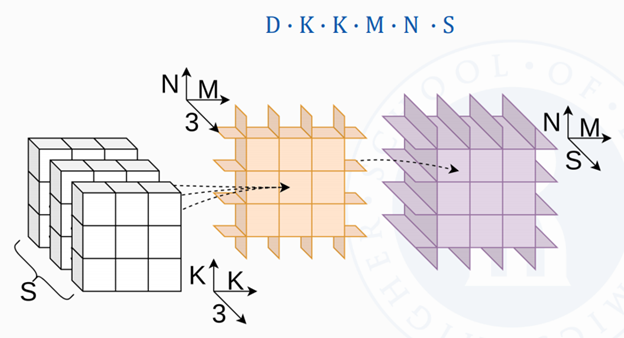
\includegraphics[width=\linewidth]{\picPath/arc_1.png}
  \caption{Визуализация трехмерной операции свертки}
  \label{fig:arc_1}
  \end{center}
\end{figure}

Теперь давайте попробуем адаптировать ту идею разделения сверток, которая была представлена выше в двумерном случае. На первом этапе у нас вместо одной свертки размера $D \times K \times K$ будет $D$ сверток двумерных размера всего лишь $K \times K \times 1$. Каждую конкретную свертку мы применим независимо к своему каналу в изображении. То есть если в изображении было три канала, у нас будет три свертки двумерные размера $K \times K$. 

Мы параллельно и независимо их применяем и получаем по итогу $D$ каналов, но уже с примененными двумерными свертками. После этого осталось этот результат размера $D \times N \times M$ свернуть в один слой, и для этого мы используем отделенную от нашей оригинальной свертки свертку размера $D \times 1 \times 1$. Она будет схлопывать обратно наши независимые слои, которые мы посчитали на предыдущем шаге. 

Если же мы теперь хотим сделать $S$ каналов по итогу, то нам вместо всей операции нужно будет $S$ раз применить последнюю свертку размера $D  \times 1 \times 1$. Такие свертки получили название "Depthwise Separable Convolutions", то есть сверки как бы разделяемые по глубине. На рисунке 1.11 изображен алгоритм выполнения такой свертки.
\begin{figure}[H]
\begin{center}
  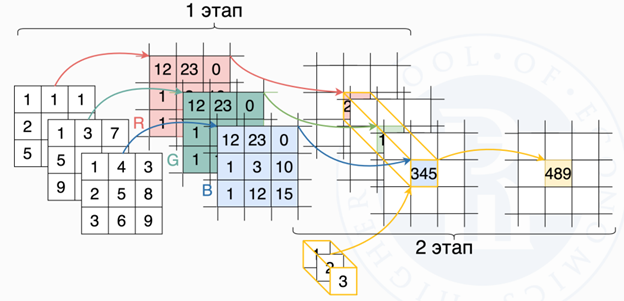
\includegraphics[width=\linewidth]{\picPath/arc_2.png}
  \caption{Визуализация depth-wise свертки}
  \label{fig:arc_2}
  \end{center}
\end{figure}
Давайте посчитаем количество перемножений. В первом случае у нас есть $D$ сверток размера $K \times K$, итого  $D \times K \times K$ операции, умножить на $N \times M$, то есть на количество пикселей в нашем изображении. Это мы сделали на первом этапе. На втором этапе нам нужно применить свертку размера $D$ к изображению $N \times M$, то есть сделать $D \times N \times M$ операций, и после этого сделать это $S$ раз. Складывая все эти числа, мы получаем итоговую формулу (1.11):
\begin{equation}
K\cdot K\cdot N\cdot M\cdot D + D\cdot N\cdot M\cdot S = N\cdot M\cdot D\cdot (K\cdot K + S)    
\end{equation}

Если взять какие-то конкретные числа:
$N=256, M=256, S=64, K=3, D=10$, тогда получим:\\
Обычные свертки:  $103\cdot 3\cdot 256\cdot 256\cdot 64 = 337$млн\\
разделяемые: $256\cdot 256\cdot 10\cdot (3\cdot 3 + 64)  = 47$млн

Мы смогли уменьшить количество перемножений почти в 8 раз, при этом количество параметров стало меньше. На основе таких сверток строилась архитектура MobileNet и это основной принцип который помог MobileNet стать легковесной моделью.

\subsection{Inception}
\textbf{Receptive field} - это размер карты характеристик, вычисляемой с помощью сверточного ядра, что в действительности и является размером ядра. Если необходимо извлечь данные с большим воспринимающим полем с высокой точностью, следует применять каскадные уровни, как показано на изображении 1.12. 

Однако можно пойти другим путем и вычислить паралельно разные свертки с разным размером ядра. Архитектурный блок Inception сети расширяет ширину сети с помощью четырех разных фильтров. Это позволяет увеличить поле воспримчивости сети и при этом значительно сократить количество вычислений. В дополнении конкатенированный результат работает лучше, чем один сверточный слой при одинаковых вычислительных нагрузках. На рисунке 1.13 изображен Inception блок
\begin{figure}[H]
\begin{center}
  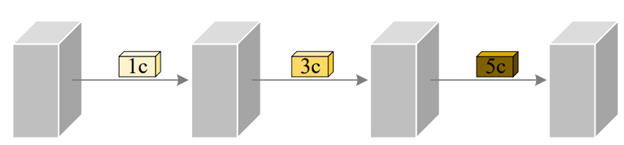
\includegraphics[width=\linewidth]{\picPath/arc_3.png}
  \caption{Каскадные свертки для увеличения воспринимающего поля нейронной сети.}
  \label{fig:arc_3}
  \end{center}
\end{figure}
\begin{figure}[H]
\begin{center}
  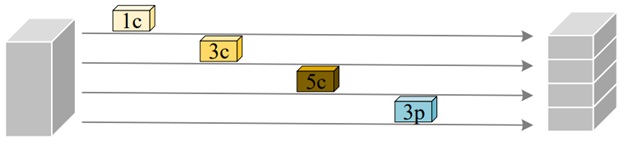
\includegraphics[width=\linewidth]{\picPath/arc_4.png}
  \caption{Inception блок}
  \label{fig:arc_4}
  \end{center}
\end{figure}
\subsection{EfficientNet}
Авторы EfficientNet предлагают использовать поиск нейронной архитектуры посредством NAS алгоритма для построения эффективной базовой архитектуры сети EfficientNet-b0. Она достигает 77.3\% точности на датасете ImageNet, при этом используя в 5 раз меньше параметров, чем ResNet50, который достигает точности в 76\%. Далее авторы предлагают масштабирование сети, посредством трех коэффициентов, отвечающих за ширину, глубину и пространственное разрешение сети.

Основным строительным блоком этой сети является MBConv, к которому добавлена операция, так называемого сжатия и возбуждения. Эта операция помогает в какой-то степени отфильтровать карты характеристик по значимости, перевзвешивая их.

MBConv аналогичен инвертированным остаточным блокам (Inverted Residuals), используемых в MobileNet V2 и V3. Карты активации входных данных сначала расширяются с использованием сверток $1 \times 1$ для увеличения глубины. За этим следуют разделяемые свертки $3 \times 3$ и точечные свертки $1 \times 1$, которые уменьшают количество каналов в выходной карте функций. Таким образом, получается инвертированный bottleneck. Эта структура помогает уменьшить общее количество требуемых операций, а также размер модели. На изображении 1.14 представлен Inverted Residual блок.

Сверточную нейронную сеть можно масштабировать в трех измерениях: глубина, ширина, разрешение. Глубина сети соответствует количеству слоев в сети. Ширина связана с количеством нейронов в слое или, что более уместно, с количеством фильтров в сверточном слое. Разрешение - это просто высота и ширина входного изображения.

\begin{figure}[H]
\begin{center}
  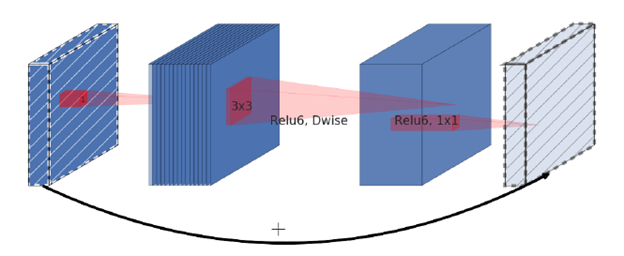
\includegraphics[width=\linewidth]{\picPath/arc_5.png}
  \caption{Inverted Residual блок}
  \label{fig:arc_5}
  \end{center}
\end{figure}

Увеличение глубины за счет применения большего количества сверточных слоев позволяет сети изучать более сложные функции. Однако более глубокие сети, как правило, страдают от исчезающих градиентов и их трудно обучать. Хотя новые методы, такие как пакетная нормализация и пропуск соединений (residual connection), эффективны для решения этой проблемы, эмпирические исследования показывают, что фактический выигрыш в точности достигаемый только за счет увеличения глубины сети быстро исчезает. Например, Resnet-1000 обеспечивает ту же точность, что и Resnet-100, несмотря на все дополнительные слои.

Масштабирование ширины сетей позволяет слоям изучать более мелкие объекты. Эта концепция широко использовалась во многих работах, таких как Wide ResNet и Mobile Net. Однако, как и в случае увеличения глубины, одно лишь увеличение ширины не позволяет сети изучать сложные функции, что приводит к снижению прироста точности.

Более высокое входное разрешение обеспечивает более подробную информацию об изображении и, следовательно, увеличивает способность модели рассуждать о более мелких объектах и извлекать более детальные узоры. Но, как и другие масштабные изменения, это тоже само по себе имеет ограниченный прирост точности.

Авторы предлагают простой, хотя и эффективный метод масштабирования, который использует составной коэффициент $ \phi $ для единообразного масштабирования ширины, глубины и разрешения сети как представлено в уравнении 1.11.

$\phi$ - определяется пользователем, это глобальный коэффициент масштабирования (целое число), который контролирует количество доступных ресурсов, тогда как $\alpha$, $\beta$ и $\gamma$ определяют, как “распределить” эти ресурсы на глубину, ширину и на пространственное разрешение сети соответственно. FLOPS (количество операций с плавующей точкой в секунду) сверточной сети пропорциональны $d$, $w^2$, $r^2$, поскольку удвоение глубины удвоит FLOPS, в то время как удвоение ширины или разрешения увеличивает FLOPS почти в четыре раза. Таким образом, масштабирование сети с использованием уравнения 1.11 увеличит общее количество FLOPS на $(\alpha \cdot \beta^2 \cdot \gamma^2) ^ \phi$. Следовательно, чтобы гарантировать, что общее количество FLOPS не превышает $2 ^ \phi$, применяется ограничение $(\alpha \cdot \beta^2 \cdot \gamma^2) \approx 2$. Это означает, что если у нас вдвое больше доступных ресурсов, мы можем просто использовать составной коэффициент 1 для масштабирования количества операций в секунду в 2 раза.
\begin{equation}
\begin{split}
\text{глубина:} d = \alpha^\phi\\
\text{ширина}: w = \beta^\phi\\
\text{разрешение}: r = \gamma^\phi\\
\text{при ограничениях}: \alpha \cdot \beta^2 \cdot \gamma^2 \approx 2\\
\alpha \geq 1, \beta \geq 1, \gamma \geq 1
\end{split}
\end{equation}

Параметры - $\alpha$,$\beta$ и $\gamma$ - можно определить с помощью жадного поиска, установив $\phi$ = 1 и найдя параметры, которые приводят к наилучшей точности. После того, как эти параметры найдены, их можно зафиксировать, а составной коэффициент $\phi$ можно увеличить, чтобы получить более крупные, но более точные модели. Так построены EfficientNet-B1 - EfficientNet-B7, с целым числом в конце названия, указывающим значение составного коэффициента.
\section{дистилляция знаний}
\subsection{Пример дистилляции знаний}

В этой секции мы рассмотрим на примере задачи классификации такой метод, как дистилляция. Когда мы обучаем большую нейронную сеть, мы, по сути,  аккумулируем гигантское количество информации про ту или иную предметную область. Вся эта информация зашита где-то в глубинных слоях этой нейронной сети и позволяет ей принимать какие-то решения. Однако, сами эти знания, которые находятся внутри нейросети, мы практически никогда не используем. Нас чаще всего интересует конкретный ответ данной сети на конкретный вопрос, то, как она “думала” и как она пришла к этому ответу нас скорее всего не интересует. Если же взглянуть на маленькие нейронные сети, их количество параметров может просто не позволить этим моделям хорошо обучиться и понять структуру предметной области, поэтому они обучаются хуже и дают хуже качество с точки зрения целевой метрики. Возникает логичная мысль: а можем ли мы как-то использовать все эти скрытые знания, которые зашиты внутри большой модели (внутри модели учителя), и передать их в маленькую модель (в модель ученика)? 

Давайте посмотрим на последний слой какой-либо нейронной сети. Чаще всего мы можем увидеть там какой-то полносвязный слой, который дальше передается в функицию SoftMax, которая превращает эти выходы в вероятности ответов. На рисунке 1.15 представлена визуализация этого процесса.
\begin{figure}[H]
\begin{center}
  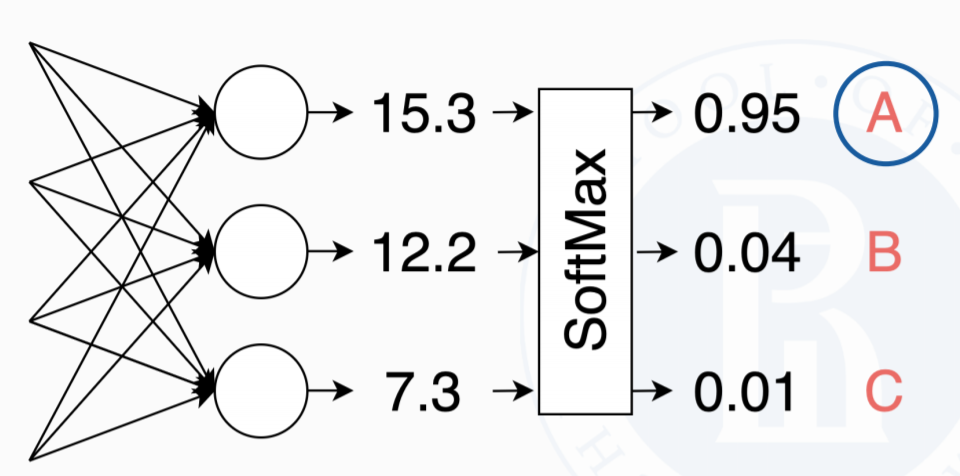
\includegraphics[width=\linewidth]{\picPath/distil_1.png}
  \caption{Визуализация последнего слоя нейронной сети и операции SoftMax}
  \label{fig:distil_1}
  \end{center}
\end{figure}

В данном конкретном случае у нас есть какая-то нейронная сеть и три класса, и нейронная сеть выдает три числа, которые являются вероятностями принадлежности к тому или иному классу. Видно, что так как для класса А — вероятность составляет 0.95, то есть на 95\% процентов нейронная сеть уверена, что это класс А. 
Однако, стоит заметить, что и про класс B и C — она тоже что-то “сказала”. А именно, что входные данные похожи так же на класс Б, но всего лишь на четыре процента, и на класс C — на один процент. Именно это и можно назвать так называемой интуицией модели, то есть то, как она вообще смотрит на текущий пример данных и как она думает, с какой вероятностью представлен тот или иной класс. 

Эту информацию можно попробовать передавать маленькой нейронной сети вместе с правильными ответами. Таким образом, мы можем надеяться, что добавление подобной информации, выходного распределения для всех классов от большой модели, которая хорошо понимает данные, в маленькую — позволит ей быстрее сориентироваться в том пространстве данных, которое мы ей передаем, и лучше и быстрее обучиться. 

Остается последний вопрос: как технически это реализовать? Мы должны сделать более сложную функцию ошибки, которую нам потребуется минимизировать в процессе обучения. У нас есть размеченные данные, на которых мы посчитаем стандартную ошибку классификации посредством кросс-энтропии и просто к этой ошибке (через оператор плюс) мы добавляем другую ошибку — ошибку дистилляции. В качестве ошибки дистилляции берут расстояние (расхождение, дивергенция) Кульбака — Лейблера. Для дискретных вероятностных распределений $P$ и $Q$ с числом элементарных событий n данное расстояние можно представить как (1.13).
\begin{equation}
D_{KL}(P||Q)=\sum_{i=1}^{n}p_ilog\frac{p_i}{q_i}
\end{equation}
где\ \ $P$ – постулируемое априорное распределение\\
$Q$ – предполагаемое, проверяемое распределение

Значение функционала можно понимать как количество неучтённой информации распределения $P$, если $Q$ было использовано для приближения $P$. Данная мера расстояния в теории информации также интерпретируется как величина потерь информации при замене истинного распределения $P$ на распределение $Q$.
Нужно конечно еще добавить, что есть некоторые нюансы, которые также нужно учитывать. Если у нас очень мощная модель и мы ее очень хорошо натренировали — скорее всего она будет слишком уверена в своих ответах, такая проблема в литературе называется overconfidence, она является прямой причиной переобучения. Другими словами, если  мы дадим какое-то изображение сети и она выдает, что с вероятностью 99\% или даже с вероятностью 100\% — это картинка класса А, по сути она выдает практически те же результаты, что и просто правильный ответ из размеченных данных. Какой-то дополнительной информации здесь можно не получить, потому что она не будет отличаться от того, что мы и так подаем на вход нашей маленькой сети. 

Для предотвращения данной проблемы есть такой подход, как нагретый SoftMax. В целом это самый обычный SoftMax с одним исключением: мы все входные данные дополнительно делим на параметр $T$ (на параметр температуры), как показано в уравнении (1.14).
\begin{equation}
\frac{exp(\frac{z_i}{T})}{\sum_{j}^{}exp(\frac{z_j}{T})}
\end{equation}
где\ \ $z_i$ – это логитсы (выходы) модели\\
$T$ – температура

Данный прием позволяет сгладить выходное распределение моделей и из почти one-hot  распредления получить более мягкое. Например, у нас есть нейронная сеть, которая выдает результаты 98\% для класса А и всего 2\% — для класса В, и это можно считать слишком уверенным ответом. Теперь разделим все выходы до SoftMax на параметр t (в данном примере t равен 5) и видим, что  распределение ответов немножко смягчилось, то есть вероятностное распределение распределилось по другим классам. На рисунке 1.16 представлена визуализация действия нагретого SoftMax.

Ошибку для правильных ответов, на размеченных данных, мы оставляем, как есть, а ошибку дистилляции, то есть когда мы будем сравнивать распределение сети-студента и сети-учителя, мы будем прогонять дополнительно через нагретый SoftMax, для более глубокого обмена скрытой в более ресурсоемкой модели информации. Важно отметить, что нагретый SoftMax нужно использовать и для сети-учителя и для сети-ученика для вычисления функции потерь дистилляции.

В этом и заключается базовая идея дистилляции, однако ее можно дополнительно модифицировать, чтобы достигать какого-то лучшего качества и, может быть, экспериментировать с различными другими подходами. Например, мы можем дистиллировать не только последний слой, а еще какой-то более глубокий. 

Пусть есть какая-то одна нейросеть и другая нейросеть поменьше, они имеют согласованную структуру, то есть обе представители одной архитектуры, просто вторая физически меньше, то мы можем пытаться сравнивать точно таким же образом через нагретый SoftMax какие-то более глубокие слои в первой и во второй нейросети. На рисунке 1.17 можно видеть схематичную визуализацию этого процесса.

\begin{figure}[H]
\begin{center}
  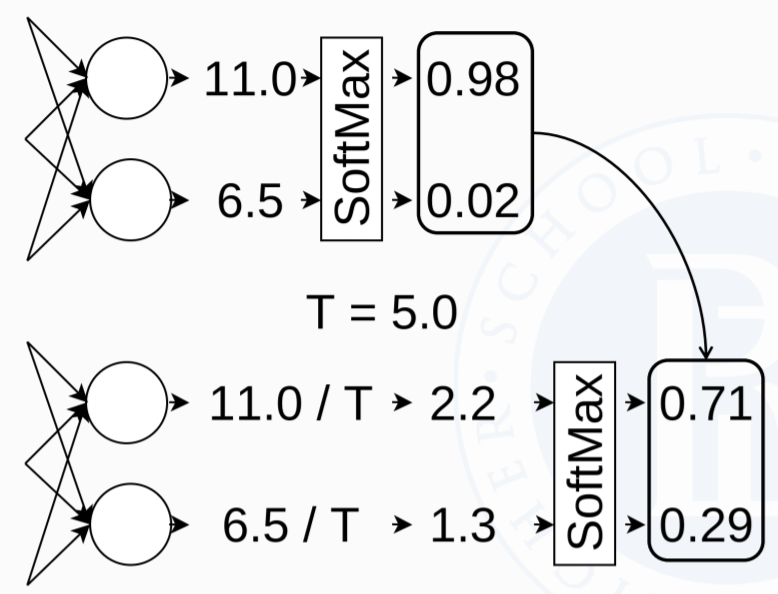
\includegraphics[width=0.8\linewidth]{\picPath/distil_2.png}
  \caption{Визуализация действия нагретого SoftMax}
  \label{fig:distil_2}
  \end{center}
\end{figure}


\begin{figure}[H]
\begin{center}
  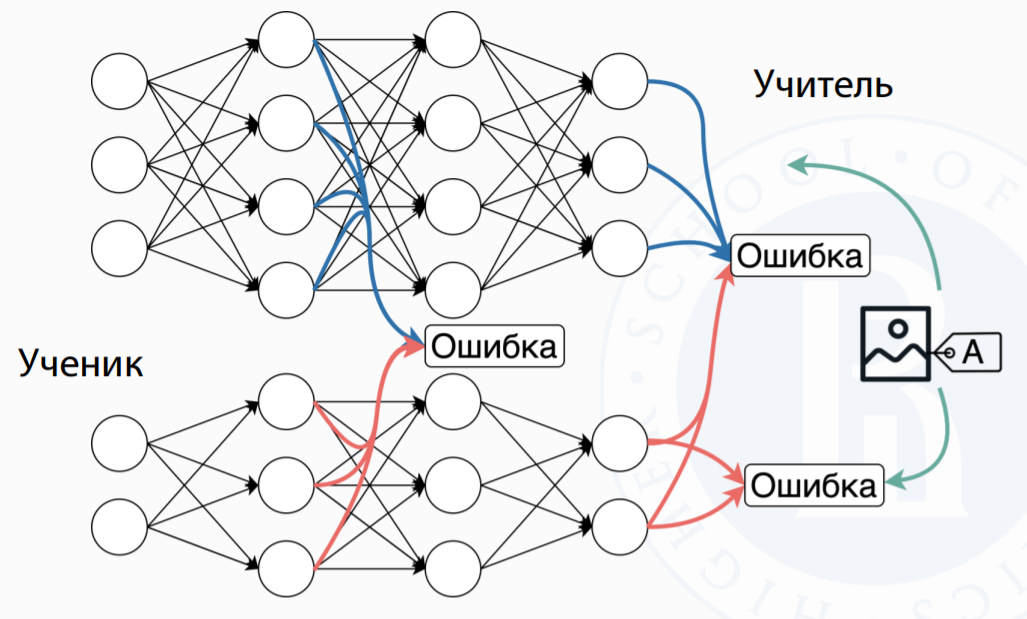
\includegraphics[width=0.8\linewidth]{\picPath/distil_3.png}
  \caption{Визуализация дистиллирования знаний с более глубоких слоев}
  \label{fig:distil_3}
  \end{center}
\end{figure}
Также можно применить этот подход к автоматической разметки данных следующим образом: пусть у нас есть уже какие-то размеченные данные и на них мы классически обучаем нашу модель. Однако могут быть еще и какие-то неразмеченные данные, они просто лежат и для того, чтобы их как-то задействовать, в цикле разработки продукта в компании мы бы попросили какой-то отдел разметки, чтобы они разметили эти данные, передали нам и мы их добавили в обучающую выборку. Мы могли бы попытаться использовать “знания” большой ресурсоемкой модели  для того, чтобы добавить новые данные в обучающую выборку. Тут нужно тоже отдельно упомянуть, что так как наша модель все-таки не идеальна и она не может прямо со стопроцентной точностью разметить данные, то не нужно бинализировать ее ответы, стоит использовать мягкое распределение через нагретый SoftMax. На рисунке 1.18 схематично представлен алгоритм обучения на таких полуразмеченных данных.
\begin{figure}[H]
\begin{center}
  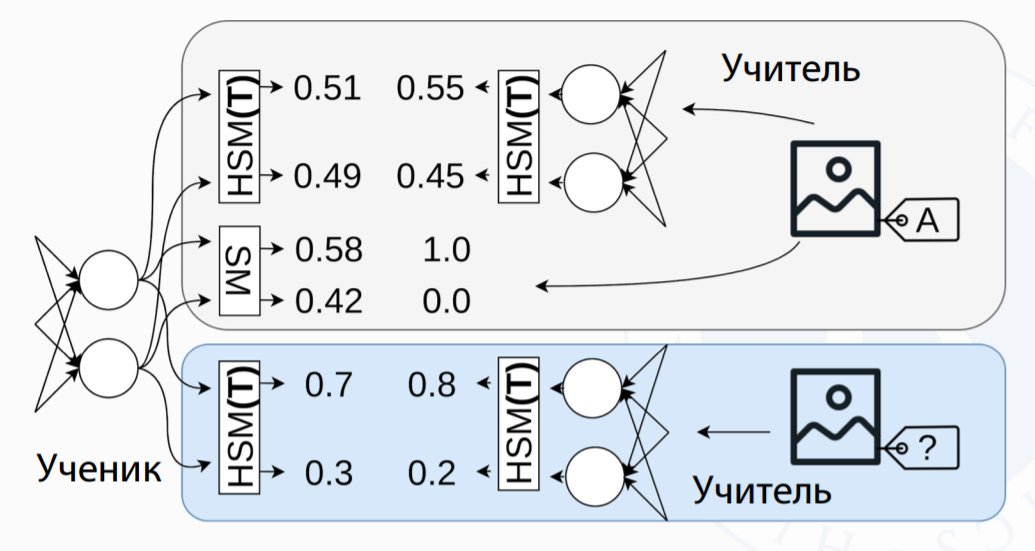
\includegraphics[width=\linewidth]{\picPath/distil_4.png}
  \caption{Визуализация обучения на полуразмеченных данных}
  \label{fig:distil_4}
  \end{center}
\end{figure}
Таким образом, используя дистилляцию, мы можем улучшить качество и скорость обучения маленькой сети, чтобы она могла быть, с одной стороны, компактной, но при этом “понимала” про данные так же много, как и более большая модель. К тому же подход дистилляции знаний может помочь при дополнительной мягкой разметки данных.

Рассмотрим, как применить процесс дистилляции знаний на практике. Наша задача взять более большую, уже предобученную модель на данных и дистиллировать знания в маленькую с точки зрения параметров сеть.
\subsection{Программная реализация дистилляции знаний}

Для примера программной реализации возьмем предоубученную нейронную сеть с более чем 2 миллионами параметров (2 669 248 параметров) для распознавания изображений. Эта модель была обучена на датасете Fashion MNIST и мы можем использовать полученные веса для дистилляции. Fashion-MNIST - это набор изображений статей Zalando, состоящий из обучающего набора из 60 000 примеров и тестового набора из 10 000 примеров. Каждый пример представляет собой черно-белое изображение с разрешением 28x28 пикселей. Всего представленно 10 классов. Мы будем использовать Fashion-MNIST для обучения нейронных сетей в данной курсовой работе, так как это небольшой по своим размерам датасет, на котором можно быстро получить результаты, а также, считается, что это более сложная задача, чем классический MNIST. Пример изображения одного из классов, а также весь код представлен в приложении А к курсовой работе.

В качестве сети-ученика возьмем сеть с двумя полносвязанными слоями с 20 нейронами: 139-20, 20-10. Посчитав количество параметров сети-ученика видим, что модель гораздо меньше первой и имеет 3.5 тысячи параметров. Также время инференса для нее значительно меньше, примерно в 3 раза. Далее посмотрим, какое качество модель выдает сама по себе. Точность составляет 82.7\%, в то время как крупная модель показывает метрику 91.2\%. Основная задача - дистрилировать знания из этой модели в более компактную модель.

Напишем функции тренировки и валидации, стандартные для фреймворка Pytorch. Мы объявим функцию \texttt{error\_and\_output} которая задает особую функцию Дивергенции Кульбака-Лейблера. Дивергенция Кульбака-Лейблера нужна, чтобы подсчитать кросс-энтропию между двумя распределениями. А именно между распределениями ответов модели-учителя и модели-ученика. После подсчета логитсов моделей учителя и ученика рассчитываем распределение вероятностей ответов сетей с помощью softmax с параметром T (нагретый софтмакс) для сети-ученика и для сети-учителя. В конце складываем ошибку ученика и взаимную кросс энтропию с соответсвующим коэффициентом альфа. Следует отметить, что этот коэффициент, а также температура получены эмпирическим путем посредством экспериментов.

Обучим нашу сеть-ученика, пользуясь знаниями сети-учителя. После тренировки видим, что что применяя дистилляцию знаний, нам удалось повысить качество маленькой модели на несколько процентов, при этом сохранив ее компактность. В таблице 1.1 представлена сводная информация по полученным метрикам на данных FashionMNIST

\begin{table}[H]
% Подпись таблицы
\caption{Результаты дистилляции знаний}
% Ссылка на таблицу
\label{table_1.1}
\begin{tabularx}{\textwidth}{|X|X|} % Столько X, сколько столбцов
\hline
Модель & Точность, \% \\ \hline
BigNet & 91.2 \\ 
ScNet baseline & 82.7 \\ 
ScNet distilled & 84.1 \\ \hline 

\end{tabularx}
\end{table}

\chapter{Прунинг и прореживание нейронных сетей}
\textbf{Отсечение сети} - важный метод как для уменьшения объема памяти, так и для оптимизации ее пропускной способности. В начале 1990-х годов были разработаны методы отсечения, чтобы сжать обученную большую сеть в меньшую сеть без необходимости переобучения. Это позволило развертывать нейронные сети на мобильных и ограниченных платформах. При прунинге удаляются избыточные параметры или нейроны, которые не вносят существенного вклада в точность результатов. Различные методы прунинга предлагают как именно выбрать это условие по которому  веса классифицируются как ненужные и избыточные.  

Так как мы убираем некоторую часть весов это снижает вычислительную сложность алгоритма. Многие исследования подтверждают, что если сокращенные сети повторно обучить, то это может позволить избежать предыдущих локальных минимумов, возникших при тренировке, которые не позволяют сети достичь максимальной точности. Исследования по сокращению сети начались в начале 1990-х годов и были разделены на методы расчета чувствительности и так называемые иметоды штрафных санкций (penalty-term methods).

Сейчас наблюдается значительные интерес к данной теме и последние работы в этой области показывают улучшения как для отдельных категорий сокращения сети, так и для их дальнейшей комбинации. Современные методы отсечения можно классифицировать по различным аспектам, включая:
\begin{itemize}
    \item структурированное и неструктурированное отсечение в зависимости от того, является ли отсекаемая сеть симметричной или нет
    \item отсечение целых нейронов или связей между нейроными
    \item статическое и динамическое отсечение. 
\end{itemize}

На рисунке 2.1 показаны различия в обработке статической и динамической обрезки. При статическом прунинге все этапы выполняются в автономном режиме до инференса сети, в то время как динамическое сокращение выполняется во время обучения. Несмотря на то, что категории частично совпадают, в этой главе мы будем использовать статическое и динамическое отсечение для классификации методов прунинга сети. 

\begin{figure}[H]
\begin{center}
  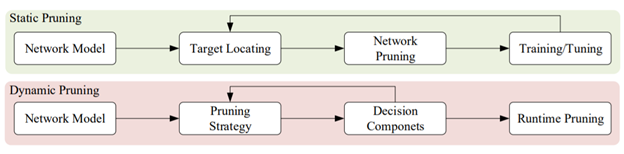
\includegraphics[width=\linewidth]{\picPath/pruning_1.png}
  \caption{Схемы статического и динамического отсечения}
  \label{fig:pruning_1}
  \end{center}
\end{figure}

\begin{figure}[H]
\begin{center}
  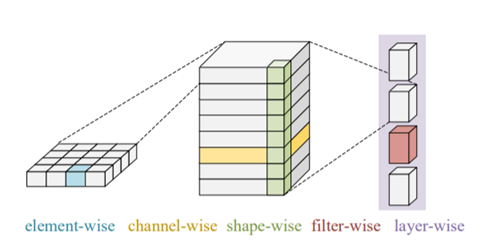
\includegraphics[width=0.8\linewidth]{\picPath/pruning_2.png}
  \caption{Различные виды отсечения}
  \label{fig:pruning_2}
  \end{center}
\end{figure}
Отсечение может происходить по элементам, строкам, по столбцам, по фильтрам или по слоям. На рисунке 2.2 показаны возможные варианты отсечения. Обычно применение element-wise подхода оказывает наименьшее влияние на разреженность сети. На рисунке разреженность сети уменьшается слева направо.
Независимо от типа прунинга, данную операцию можно описать математически как показано в уравнении 2.1:
\begin{equation}
    \arg \min_{p} L = N(x;W) - N_p(x;W_p)
\end{equation}
где $N_p(x;W_p) = P(N(x;W))$\\
$ P(\cdot) $ - функция прунинга\\
$L$ представляет собой некоторую функцию меры точности нейронной сети \\
$N$ - исходная нейронная сеть\\
$W$ - исходные веса нейронной сети\\
$N_p$ - нейронная сеть после прунинга

Задача любого подхода к отсечению сетей это поиск такой функции прунинга $P(.)$, чтобы минимизировать потерю в качестве после отсечения и при этом как можно лучше проредить сеть.

\section{Статический прунинг}
\textbf{Статический прунинг} – это метод оптимизации сети, при котором удаляются ее параметры после обучения и до развертывания этой сети у клиента. Во время инференса никакого дополнительного прунинга не производится. 
Статический прунинг, как правило, имеет 3 части:
\begin{itemize}
    \item Выбор параметров для отсечения по какому-то критерию
    \item Выбор метода отсечения
    \item Опционально, дотренировка сети после этой операции
\end{itemize}

Дотренировка сети может увеличить получаемое качество сети по сравнению с оригинальной версией, но и может потребовать значительных ресурсов и времени для последующей тренировки.

\subsection{magnitude-based pruning}
Один из первых методов обрезки сетей – это метод перебора. В этом методе выполняется поэлементный обход всей сети и удаление тех весов, которые не влияют на точность.

Недостатком такого подхода, естесственно, является большая временная сложность данного алгоритма и большое пространство решений. Типичная метрика для определения какие параметры можно обрезать является $l_p$ норма. $l_p$ норма вектора, который содержит $n$ элементов можно выразить математически как показано в уравнении (2.2):
\begin{equation}
    \left \|X_p  \right \| = (\sum_{i=1}^{n}\left | x_i \right |^p)^{\frac{1}{p}}
\end{equation}

Такой подход называется magnitude-based. Было предложено и широко признано, что натренированные веса с большими значениями более важны, чем натренированные веса с меньшими значениями. Это наблюдение является ключом к данному методу.
Методы отсечения, основанные на величине, стремятся идентифицировать ненужные веса или функции, чтобы удалить их при применении сети для задачи. Ненужные значения могут быть удалены либо в ядре свертки, либо на карте активаций. Самый интуитивно понятный метод отсечения, основанный на величине - это отсечение всех весов с нулевым значением или всех весов в пределах некоторого порога по абсолютному значению.

Ян Лекун еще в 1990 году предложил метод оптимального повреждение мозга (OBD) для удаления отдельных несущественных весов. Используя вторую производную (матрицу Гессе) функции потерь, этот метод статической обрезки снизил параметры сети на четверть. Для упрощенного вычисления производной, функция OBD рассматривалась при трех предположениях: 
\begin{itemize}
    \item квадратичная - функция стоимости почти квадратичная
    \item экстремальная – обрезка делается после схождения сети
    \item диагональная – суммирует отдельные производные весов как результат их совместного следствия
\end{itemize}

Это исследование также показало, что разряжение нейронной сети может предоставить возможности для повышения ее производительности. Позднее был предложен метод Optimal Brain Surgeon (OBS), расширенная OBD с аналогичным методом вычисления производной второго порядка, но без диагонального допущения в OBD. OBS рассматривает матрицу Гессе как недиагональную для большинства случаев. OBS повысил точность прунинга с 90\% сокращением, особенно для сетей XOR.

Эти ранние методы уменьшили количество связей между нейронная на основе второй производной функции потерь. Они также предложили методы, основанные на методе матрицы Гессе, при которых такая обрезка сети будет показывать более высокую точность, чем magnitude based прунинг. Но современные сети имеют намного больше праметров, чем сети в те времена. Например, GPT-3 содержит 175 миллиардов параметров, тогда как VGG-16 содержит 133 миллиона. Вычисление матрицы Гессе во время тренировки потребует вычислительной сложности порядка $О(W^2)$ и для GPT-3 такая сложность недосягаема на текущий момент. Именно поэтому сейчас используют в основном различные алгоритмы основанные на величиние значений нейронной сети.

Давайте посмотрим на конкретный пример: пусть у нас есть нейросеть и нам нужно понять, какие здесь веса лишние, а какие нужно оставить и они будут отвечать за корректную работу алгоритма. Для того, чтобы думать о том, какой из весов является важным, а какой нет, можно смотреть на очень простой критерий: можно смотреть на модуль коэффициентов, привязанных к конкретной связи.
\begin{figure}[H]
\begin{center}
  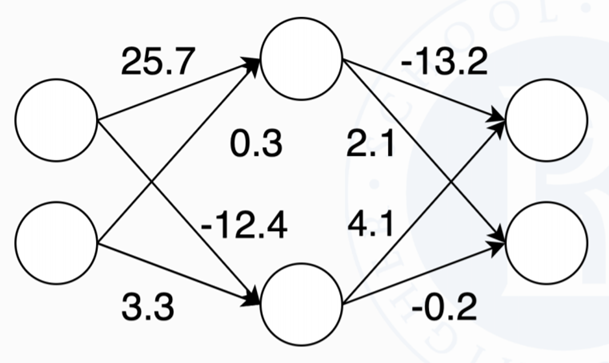
\includegraphics[width=0.7\linewidth]{\picPath/pruning_3.png}
  \caption{Пример полносвязанной нейронной сети}
  \label{fig:pruning_3}
  \end{center}
\end{figure}

На схематичном изображении 2.3 приведена простая полносвязанная сеть, у этой сети есть три связи с коэффициентами: 25, - 13 и - 12. Это довольно большие значения относительно всех представленных весов в этой сети и поэтому ожидается, что если мы их удалим,то точность сильно просядет и сеть перестанет хорошо выполнять поставленную перед ней задачу.

Однако в этой же сети есть и другие связи, например, с коэффициентом -0.2 и 0.3. 
Эти значения относительно не очень большие,  поэтому можно ожидать, что если мы удалим их сети, то есть заменим на 0, то не очень много что поменяется в работе сети и она все также будет хорошо предсказывать изначальный ответ, однако уже без лишних параметров.
 
Итак, будем удалять из нашей нейросети веса с наименьшим значением по модулю; в данном конкретном примере возьмем вес с коэффициентом - 0.2 и так, как он самый маленький по модулю, удалим его. Однако стоит отметить, что такое удаление весов не пройдет бесследно и мы можем ожидать небольшую потерю в качестве.  Поэтому, чтобы восстановить предсказательную способность нашей сети, применяют процесс дотренировки на оставшихся параметрах. Мы ожидаем, что сеть все-таки уже хорошо обучена, и мы не будем очень долго ее дообучать и проведем несколько эпох для того, чтобы оставшиеся связи как бы взяли на себя ту роль, которая лежала на удаленных коэффициентах.

После того как мы дообучили оставшуюся нейросеть, мы можем продолжать наш алгоритм, то есть продолжать удалять веса с наименьшим коэффициентом. Удаляем снова и после этого проводим еще один этап дообучения нейросети. Таким вот образом мы будем удалять веса и восстанавливать качество дообучением до тех пор, пока качество не будет падать драматически. 

Такой алгоритм называется итеративным прунингом. Однако если мы будем удалять только по одному весу — это будет очень долгий процесс. Вместо этого можем использовать более грубый подход: можем удалять, например , по 10 процентов сети. Тогда за девять шагов мы бы могли теоретически удалить 90 процентов сети, не потеряв сильно в качестве. Весь алгоритм представлен на изображении 2.4.

Мы рассмотрели возможный алгоритм с element-wise подходом. Как уже было сказано выше у этого алгоритма также есть вариации. Мы можем прореживать веса целиком в сети, а можем делать это конкретно по слоям, то есть смотреть не на самый маленький коэффициент по абсолютному значению внутри всей сети, а на самый маленький в конкретном слое. Можно удалять не какие-то отдельные элементы, а целые нейроны, слои или фильтры (filter pruning). При таких подходах в основном используется $L_p$ норма (в частности $L_1$) для удаления фильтров, которые не влияют на точность классификации, а также удаляются связанные с этим фильтром карты характеристик.  Такая работа приводит к снижению затрат на инференс на 34\% для VGG-16 и на 38\% для ResNet-110 при этом увеличивая точность на 0.75\% и 0.02\% соответственно при экспериментах на CIFAR-10. Алгоритм же выбора значимых или не значимых нейронов можно схематично изобразить как показано на рисунке 2.5.

Большинство методов отсечения сетей предпочитают измерение веса, а не активаций для критерия прунинга. Однако активации также могут быть индикатором для сокращения соответствующих весов. Средний процент нулей (APoZ)  был введен, чтобы судить, влияет ли та или иная выходная карта активации на конечный результат. Некоторые функции активации, в частности функции Rectified linear utit (ReLU) могут приводить к высокому проценту нулей в активациях и, таким образом, поддаваться к прунингу. 

\begin{figure}[H]
\begin{center}
  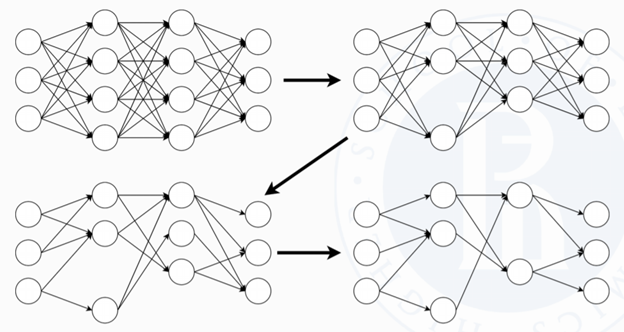
\includegraphics[width=\linewidth]{\picPath/pruning_4.png}
  \caption{Схемы статического и динамического отсечения}
  \label{fig:pruning_4}
  \end{center}
\end{figure}


\begin{figure}[H]
\begin{center}
  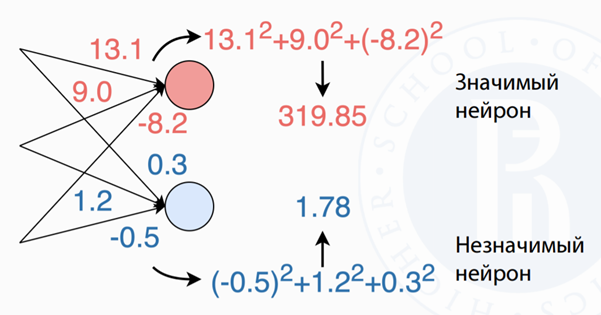
\includegraphics[width=\linewidth]{\picPath/pruning_5.png}
  \caption{Схемы статического и динамического отсечения}
  \label{fig:pruning_5}
  \end{center}
\end{figure}

Уравнение 2.3 демонстрирует определение APoZ для $c$-го нейрона на $i$-ом слое.
\begin{equation}
    APoZ_c^{(i)} = APoZ(O_c^{(i)}) = \frac{\sum_{k=0}^{N}\sum_{j=0}^{M}f(O_{c,j}^{(i)}(k)=0)}{N \times M}
\end{equation}
где $O_c^{(i)}$ - обозначает активацию\\
$N$ - количество валидационных изображений\\
$M$ - пространственное разрешение карты активации\\
$f(true) = 1;\ f(false) = 0$
\subsection{Regularize-based sparsity}
Выполнение отсечения по фильтрам с порогом из суммы абсолютных значений будет напрямую использовать преимущество структурной сети. Таким образом, коэффициент сокращения сети положительно коррелирует с процентом нулей в ядре свертки, который может быть повышен с помощью наложенных ограничений на веса в процессе обучения, эта техника известна в литературе как регуляризация. Исходя из этого строится прунинг на основе штрафа. При прунинге на основе штрафов цель состоит в том, чтобы изменить функцию ошибок или добавить дополнительные ограничения, известные как условия смещения (bias terms), в процесс обучения. 

Штрафное значение используется для обновления некоторых весов до нулевых или близких к нулю значений. Затем эти значения удаляются. В частности существует метод, исследованный в конце 80х, который использует уменьшение веса при обратном распространении ошибки, чтобы определить, нужно ли обрезать нейрон. Веса с наименьшим значением заменяются нулями. Остаточные нулевые веса после обучения затем используются для отсечения ненужных нейронов.

Позднее в качестве штрафа было введено LASSO. LASSO уменьшает соответствующие веса наименее значимых признаков, это также ведет к увеличению разреженности. Поэлементное сокращение может привести к неструктурированной сетевой организации. Это приводит к разреженным матрицам весов, которые неэффективно выполняются на процессорах. Кроме того, их обычно трудно сжать или ускорить без специализированной аппаратной поддержки. 

Group LASSO смягчает эту неэффективность, используя метод структурированной отсечения, который удаляет целые группы нейронов, сохраняя структуру организации нейронной сети. Групповой LASSO предназначен для того, чтобы все переменные, отсортированные в одну группу, можно было либо включить, либо исключить как единое целое. Уравнение (2.4) дает критерий для отсечения весов посредством этого метода
\begin{equation}
    \arg \min_{\beta\in R^p}\left \{ \left \| y - \sum_{j=1}^{J}X_j\beta_j \right \|^{2}_2 + \lambda \sum_{j=1}^{J}\left \| \beta_j \right \|_{K_j} \right \}
\end{equation}

Веса разделены на несколько групп. Ненужные группы весов удаляются с помощью выбора функций LASSO. Группы могут определяться на основе геометрии, вычислительной сложности, разреженности групп и т.д. Можно найти примеры исследований, в котором разреженность групп в направлении строк или столбцов (структурное разрежение) может использоваться для сокращения времени выполнения GEMM. SSL (structured sparsity learning) показало улучшенное время инференса на AlexNet как на CPU, так и на GPU в 5,1 раз и в 3,1 раза соответственно.

\subsection{Variational dropout}
Dropout хоть и не является специальным методом сокращения сетей, снижает количество параметров. Первоначально он был разработан как стохастический регуляризатор, чтобы избежать чрезмерного переобучения на данных. Метод случайным образом прореживает процент нейронов, обычно до 50\%. Эта операция dropout разрывает часть связей между нейронами, чтобы избежать коадаптации. Dropout также можно рассматривать как операцию, которая отдельно обучает множество подсетей и берет их среднее значение на этапе вывода. Dropout увеличивает расходы на обучение, но не влияет на время инференса. На изображении 2.6 представлено действие dropout на нейронную сеть.

\begin{figure}[H]
\begin{center}
  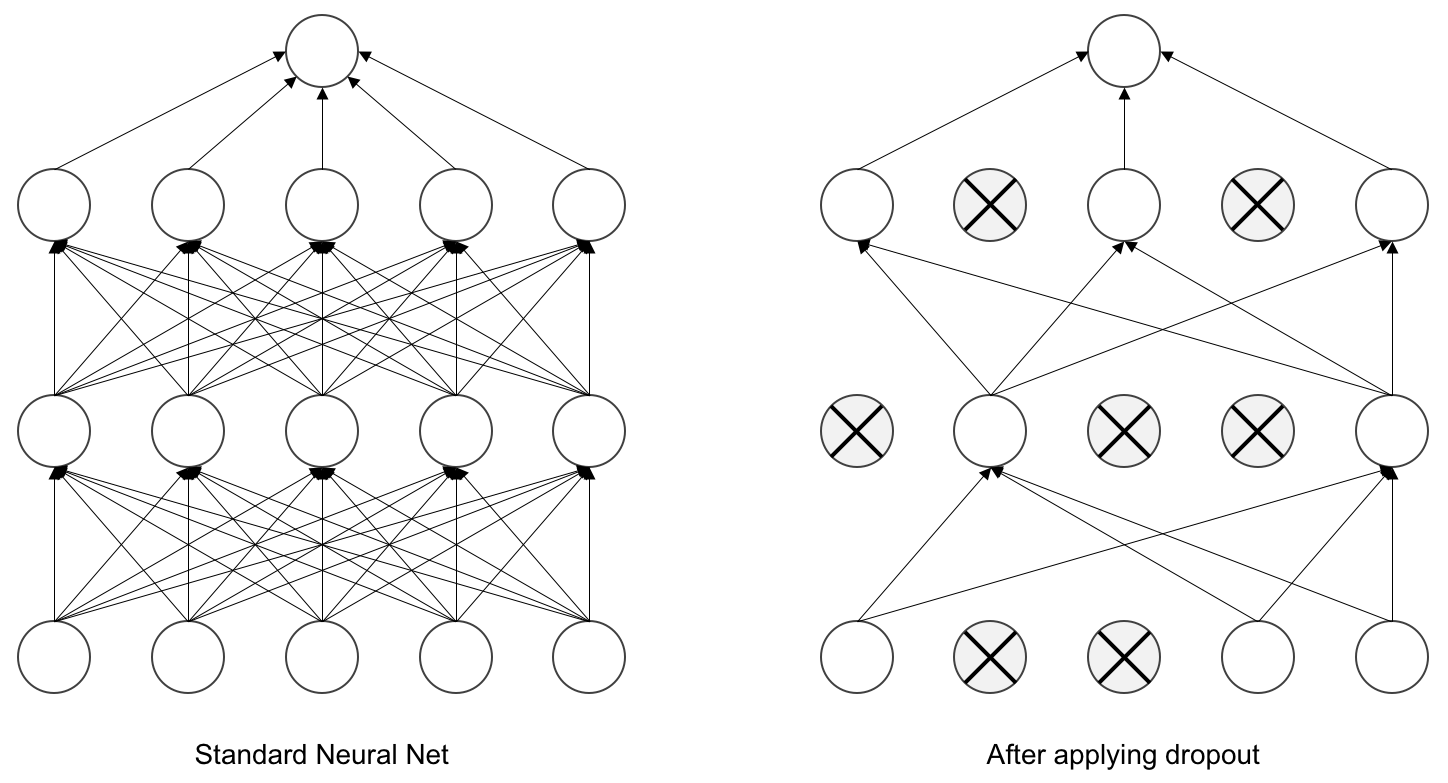
\includegraphics[width=\linewidth]{\picPath/pruning_6_1.png}
  \caption{Действие dropout}
  \label{fig:pruning_6}
  \end{center}
\end{figure}

Variational dropout добавил гиперпараметр, называемый процентом выпадения, чтобы уменьшить вес сетей, подобных VGG, в 68 раз. Во время тренировки этот гиперпараметр можно использовать для определения отдельных весов для прунинга. Это также может быть применено с другими подходами к сжатию для дальнейшего снижения веса.

\section{Динамический прунинг}
Отсеченные веса обычно невозможно восстановить. Это может привести к снижению пропускной способности сети. Восстановление утраченных возможностей сети требует значительного повторного обучения. Глубокое сжатие потребовало бы миллионов итераций для обучения сети заново. Чтобы избежать этого недостатка, во многих подходах используются восстанавливаемые алгоритмы прунинга. Отсеченные элементы также могут быть задействованы в последующем процессе обучения и подстраиваться под сокращенную сеть. 

Существует восстанавливаемый метод прунинга с использованием матриц двоичных масок, чтобы идентифицировать, сокращается ли текущее значение веса или нет. Отсеченные веса с нормой L1 могут быть стохастически возвращены обратно в сеть. Используя этот подход, AlexNet удалось уменьшить в 17,7 раза без потери точности. Итерации повторного обучения были значительно сокращены до 14,58\% от глубокого сжатия. Однако этот тип отсечения по-прежнему приводит к асимметричности сети, усложняющей аппаратную реализацию.

Хотя метод восстановления был в какой-то мере исследован, статический прунинг навсегда разрушает исходную структуру сети, что может привести к снижению возможностей модели. После удаления и повторного обучения подход статического удаления элементов сети не может восстановить уничтоженную информацию. Кроме того, наблюдения показывают, что важность связывания нейронов не зависит от входных данных.

Динамическое отсечение выполняется во время обучения, принимается решение какие слои, каналы или нейроны не будут участвовать в дальнейшей деятельности нейронной сети. Динамический прунинг может преодолеть ограничения статического прунинга за счет изменения входных данных, потенциально сокращая вычисления и пропускную способность. Динаический прунинг обычно не требует дотренировки. На рисунке 2.7 можно видеть обзор систем динамического отсечения. Самая важная часть - это система принятия решений, определяющая, какую часть обрезать. Связанные с этим вопросы:
\begin{enumerate}
    \item Тип компонентов решения:
    \begin{itemize}
        \item Дополнительные соединения, прикрепленные к исходной сети, используемые на этапе вывода и / или фазы обучения
        \item Характеристики соединений, которые могут быть изучены стандартными алгоритмами обратного распространения ошибки
	    \item Сеть побочных решений, которая имеет тенденцию работать хорошо, но ее часто трудно обучить
    \end{itemize}
    \item Уровень (форма) отсечения. Выбранный уровень обрезки влияет на тонкости разработки под конкретное железо:
    \begin{itemize}
        \item По каналам 
        \item По слоям
        \item По блокам
        \item По сети.
    \end{itemize}

\item Входные данные:
 \begin{itemize}
\item Однократная подача информации: подает весь датасет в систему принятия решений
\item Послойная подача информации, где окно данных итеративно подается в систему принятия решений паралельно с форвардом сети.
\end{itemize}
\item	Вычисление критерия решения:
\begin{itemize}
\item	$L_p$-норма
\item	Другие подходы
\end{itemize}
\item Сравнение оценок:
\begin{itemize}
\item	Человеческий опыт / результаты экспериментов
\item	Автоматический порог
\item	Динамические механизмы
\end{itemize}
\item Критерии остановки:
\begin{itemize}
\item	В случае послойного и отсечения по всей сети, некоторые алгоритмы отсечения намеренно оставляют слой / сеть неотсеченным
\item	Некоторые алгоритмы динамически выбирают по какому пути пропускать данные
\item	Другие же алгоритмы завершают вычисление и выводят результат прогноза. В этом случае оставшиеся слои считаются обрезанными.
\end{itemize}
\item Обучение компонента принятия решения:
\begin{itemize}
\item	Присоединенные соединения могут быть обучены вместе с исходной сетью 
\item	Вспомогательные сети обычно обучаются с использованием алгоритмов обучения с подкреплением (RL).
\end{itemize}
\end{enumerate}
\begin{figure}[H]
\begin{center}
  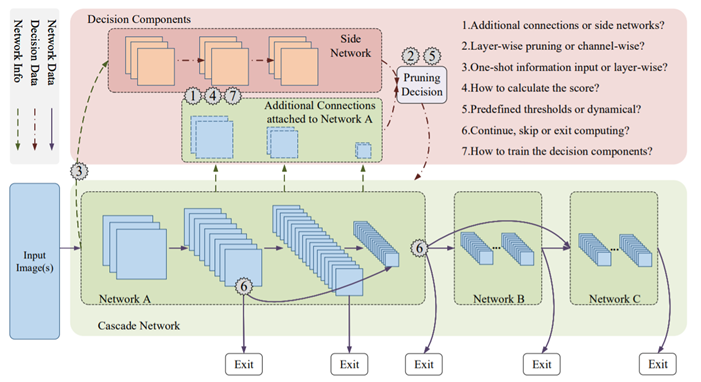
\includegraphics[width=\linewidth]{\picPath/pruning_6.png}
  \caption{Обзор систем динамического отсечения}
  \label{fig:pruning_7}
  \end{center}
\end{figure}

Для процессоров карты функций или количество фильтров, используемых для идентификации объектов, составляют большую часть использования вычислительной эффективности и полосы пропускания памяти - особенно для  depth-wise или point-wise сверток. Динамическая настройка также может применяться к статически отсеченным сетям, что потенциально дополнительно снижает требования к вычислениям и уменьшает перессылку из памяти в память.

Недостатком динамического сокращения является то, что критерии для определения элементов, подлежащих сокращению, должны вычисляться во время выполнения. Это увеличивает накладные расходы на систему, требуя дополнительных вычислений,памяти и мощности. Следует учитывать компромисс между динамическими затратами на прунинг, сокращением вычислений в сети и потерей точности. Один из методов для устранения этих проблем запрещает вычисления с нулевыми параметрами в обрабатывающем элементе (PE).

Современные подходы также предлагают более продвинутый способ понимания того, какие элементы нужно удалить, а какие нет. Одна из недавних работ позволяет делать это с помощью других нейросетей и подхода обучения с подкреплением, то есть авторы предлагают умно оценивать какие-то значимости внутри одной большой нейронной сети с помощью какой-то другой модели машинного обучения, которая может выучивать это из тех данных, которые поставляет оригинальная нейросеть. 

Таким образом, мы хотим построить какую-то одну модель, которая будет смотреть на другую и удалять уже в автоматическом режиме из нее лишние элементы. Один из таких подходов называется AutoML for Model Compression (AMC). На рисунке 2.8 изображена схема этого алгоритма.
\begin{figure}[H]
\begin{center}
  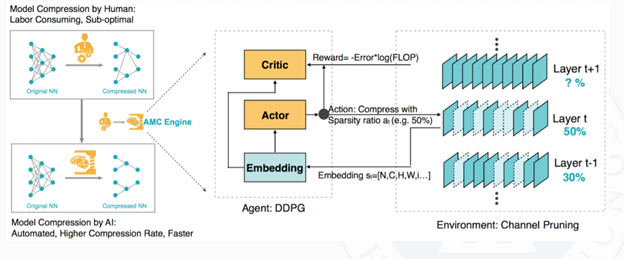
\includegraphics[width=\linewidth]{\picPath/pruning_7.png}
  \caption{AutoML for Model Compression}
  \label{fig:pruning_7}
  \end{center}
\end{figure}
Идея состоит в том, что дополнительная модель смотрит на рассматриваемую нейронную сеть и пытается удалить какие-то элементы. После этого мы запускаем оригинальную нейронную сеть и смотрим, какое качество получилось. То какое качество получилось, некоторую ее меру, мы возвращаем обратно в функцию потерь для обучения нашей вспомогательной модели. То есть простыми словами эта модель смотрит на то, хорошо у нее получилось удалить элементы или плохо, и на основе этого обучается понимать, какие элементы нужно удалять из рассматриваемой сети, а какие элементы удалять не нужно.

В оригинальной статье авторы также приводят результаты того, как работает их подход: на некоторых популярных архитектурах сжатие достигает 70\%, при этом без потери какой-либо точности. В таблице 2.1 можно видеть полученные результаты применения этого алгоритма к архитектуре MobileNet
\begin{table}[H]
% Подпись таблицы
\caption{Результаты прунинга методом обучения с подкреплением}
% Ссылка на таблицу
\label{table_1}
\begin{tabularx}{\textwidth}{|X|X|X|} % Столько X, сколько столбцов
\hline
Модель & Точность (\%) & Время работы (мс) \\ \hline
MobileNetV1 & 70.9 & 123 \\ 
MobileNetV1 - 50\% & 70.5 & 68.9 \\ 
MobileNetV2 - 70\% & 70.9 & - \\ \hline
\end{tabularx}
\end{table}

Чтобы соответствовать вычислительным ограничениям, многомасштабные плотные сети (MSDNets) были спроектированы  как адаптивная сеть, включающая два метода, один из которых – возможность генерации результатов прогнозирования во многих узлах, что позволяет ранний выход из сети; другой – ограниченный бюджет вычислений для обеспечения выхода для более  простого инференса (на более простых примерах) на раннем этапе, таким образом сохраняя вычислительные ресурсы для сложного инференса более сложных примеров. Инновационная технология MSDNets объединяет многомасштабные карты характеристик и плотную связь для обеспечения раннего выхода при сохранении более высокой точности. Классификаторы дифференцируемы, поэтому MSDNets можно обучать с использованием стохастического градиентного спуска. MSDNets обеспечивает ускорение в 2,2 раза при той же точности, что и ResNet-50, в наборе данных ImageNet.

По итогу можно сказать, что не все параметры, которые существуют в нейронной сети, 
одинаково важны для ее работы. Некоторые из этих параметров не являются необходимыми и важными для принятия решения. В целом, некоторые исследования показывают, что используя итеративное прореживание на основе прунинга фильтров и нейронов, мы можем удалять мало значимые элементы по некоторому критерию и делать нашу модель более компактной, быстрой и более осознанно решать поставленную задачу, при этом особо не уступая в производительности и эффективности сложным алгоритмам динамического прунинга.

\section{Программная реализация прореживания нейронной сети}
Для программной реализации прореживания была выбрана сеть ResNet18, адаптированная под низкое разрешение и решающая задачу классификации 10 классов. Данная сеть разработана компанией Microsoft. Сеть имеет 11.16 млн параметров и представляет собой последовательный набор Res блоков c cоединениями быстрого доступа (shortcut connections). На рисунке 2.9 схематически изображен блок такой архитектуры. Весь код был реализован с помощью низкоуровнего фреймворка для глубокого обучения PyTorch и представлен в приложении Б. 
\begin{figure}[H]
\begin{center}
  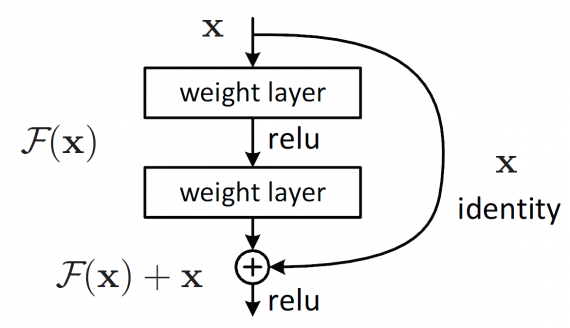
\includegraphics[width=0.8\linewidth]{\picPath/pruning_8.png}
  \caption{Res блок}
  \label{fig:pruning_8}
  \end{center}
\end{figure}

\subsection{Глобальное прореживание нейронной сети (спарсификация)}

Для того, чтобы начать оптимизировать размер сети, нам нужен инструментарий для удаления связей внутри нашей модели. В приложении Б представлена возможная реализация оберток на полносвязанный линейный и сверточный 2d слои. Идея прореживания в том, чтобы сгенирировать определенным образом бинарную маску, регулирующую какие веса мы оставляем, а какие будем отключать. Далее мы перемножим маску с весами слоя,оставляя самые важные, исходя из определенного правила при генерации этой маски.

Функция $weight\_sparse$ реализует алгоритм генерации такой маски исходя из абсолютного значения - задавая пороговое значение, вычисляем персентиль и далее зануляем только те веса, которые меньше этого значения.

Алгоритмы прунинга достаточно востребованы и поэтому в современных фреймворках уже представлен набор инструментов позволяющий проводить операцию прунинга. В методе класса нейронной сети $prune\_unstructured$ мы пробегаем по всем слоям нашей сети и применяем функцию прунинга. Метод $calc\_weights$ позволяет посчитать количество весов с учетом сгенерированных для прунинга масок. Далее реализуем простую функцию тренировки сети на тренировочных данных и функцию для тестирования на валидационных данных. Реализация этих функций поддерживает обучение и тестирование как на ЦПУ, так и на ГПУ. Далее подготовим данные для тренировки и валидации. Для наших целей будем использовать тот же набор данных, что и при реализации алгоритма дистиляции, датасет FashionMNIST, содержащий примрено 70 тысяч черно-белых изображений с разрешением 32х32. 

Первоначально обучим нашу нейронную сеть на данных перед применением алгоритма прунинга и получим метрику 93.2\%. Попробуем применить спарсификацию на полученной модели напрямую, уберем 50\% и посмотрим на просадку в качестве. Точность модели просела на 2.3\%. Результат довльно слабый. Попробуем применить другой подход, сжать сеть еще больше и при этом не допустить сильной потери в качестве

Идин из способов сжатия нейронных сетей - итеративное прореживание (Incremental Magnitude Pruning). Он достаточно ресурсоемкий, однако позволяет достаточно несложными методами добиться неплохого результата.

Будем идти с шагом, каждый раз будем отключать внутри сети несколько десятков процентов связей. После отключения, оставшиеся веса дообучим на всех данных используя одну эпоху. Ожидается, что так как мы выкинули за один раз не очень много, то оставшиеся связи "перехватят" ответственность тех слабых, которые мы только что отключили.

Таким образом за P таких итераций мы выкинем желаемое количество сети и не должны при этом потерять сильно в качестве.

Мы составим расписание для сети в виде списка и напишем более умную функцию тренировки, как показано в приложении Б. В таблице 2.2 представлены результаты спарсификации нейронной сети этим и предыдущим методами.

\begin{table}[H]
% Подпись таблицы
\caption{Результаты дистилляции знаний}
% Ссылка на таблицу
\label{table_1.1}
\begin{tabularx}{\textwidth}{|X|X|} % Столько X, сколько столбцов
\hline
Алгоритм & Точность, \% \\ \hline
baseline & 93.2 \\ \hline 
static pruning, 50\% &  90.9\\ \hline 
iterative pruning, 70\% & 93.2 \\ \hline 
iterative pruning, 90\% & 93.3 \\ \hline 
\end{tabularx}
\end{table}

Таким образом, удалось избавиться от 90\% нейронной сети, при этом качество даже немного увеличилось. Можно видеть, что итеративное прореживание намного эффективнее, но при этом требует гораздо больше ресурсов и повторного дообучения.

\chapter{Квантизация}
Квантование – это процесс аппроксимации непрерывного сигнала набором дискретных или целочисленных значений. Кластеризация и совместное использование параметров (parameter sharing) также подпадают под это определение. 

Перед тем как говорить про саму квантизацию,  давайте немного опишем в целом про то, как работают компьютеры. Какие операции они делают? По сути своей компьютер оперирует лишь какими-то числами, которые он складывает, перемножает и так далее.

Сами числа могут храниться в разных форматах. Это может быть маленький формат, типа INT8, на который уходит всего один байт, может быть полноценный INT32, где есть два-четыре байта на то, чтобы хранить информацию. Также, мы можем хранить дробные числа, так называемые числа с плавающей запятой, для которых также требуется примерно четыре байта, и они немного по-другому устроены внутри. Для каждых таких чисел, операции над ними стоят по-разному, на разных процессорах. В таблице 3.1 представлена примерная картина сколько ресурсов нам требуется в компьютере для различных операций. Это очень усредненные данные, по тому как, на разных процессорах, в разных ситуациях, с разными числами эти операции могут стоить по-разному.
\begin{table}[H]
% Подпись таблицы
\caption{Результаты прунинга методом обучения с подкреплением}
% Ссылка на таблицу
\label{table_1}
\begin{tabularx}{\textwidth}{|X|X|X|} % Столько X, сколько столбцов
\hline
Тип данных & Память (байт) & Такты процессора (такты) \\ \hline
INT8 & 2 & 1-3 \\ 
FLOAT32 & 8 & 2-8 \\ \hline
\end{tabularx}
\end{table}
Таким образом, на перемножение двух чисел в формате INT8, нам бы потребовалось два байта (по байту на число), и примерно один-три такта процессора, на FLOAT32 же, нам потребуется восемь байт, и уже где то два-восемь тактов процессора. Операции на FLOAT32 — происходят дольше и требуют больше памяти, чем на INT8. 

Давайте посмотрим на нейронную сеть. Все веса внутри нейронной сети чаще всего представляются в виде обычных дробных чисел, которые в компьютере хранятся как FLOAT32. Соответственно, возникает такая мысль, а что если мы возьмем, загрубим нейронную сеть, то есть переведем все FLOAT32 в обычные INT8. 
По идее, она должна стать быстрее, потому что операции быстрее происходят на INT8, а также занимать примерно в четыре раза меньше памяти. Остается лишь последний вопрос: "Останется ли качество такой модели приемлемым?". Рассмотрим формат числа — INT8.

Это сравнительно небольшой формат данных и он умеет хранить числа от минус 128 до 127 включительно. И из-за этого могут возникать различные проблемы при переводе FLOAT32 в INT8 каким-то простым способом. Например, в каких-то ситуациях диапазон исходных значений в формате FLOAT может оказаться очень маленьким. Если наши веса 0.23, 0.78, -0.56, -0.99, и мы просто возьмем и округлим все эти числа, то мы просто получим четыре нуля. Очевидно, что мы потеряли всю информацию. Может быть и обратная проблема, диапазон изначальных данных может быть слишком большим, если мы их округлим до ближайшего числа, которое можем закодировать с помощью INT8, то получим все значения равные 127 или -128. Тут сохраняется только знак весов, что недостаточно для сохранения информации.

Нужно каким-то более аккуратным методом, переводить изначальный диапазон FLOAT32 в диапазон целых чисел, пытаясь при этом потерять наименьшее количество информации. 

\section{Алгебра квантизации}
Для такого алгоритма существует базовое уравнение квантования чисел. Оно приведено в формуле (3.1)
\begin{equation}
X_q=f(s \times  g(X)+z)    
\end{equation}

Для того, чтобы переводить FLOAT в INT, мы будем сжимать или разжимать наше изначальное значение и немного сдвигать.  Будет два дополнительных параметра: параметр сжатия, который будет отвечать, чтобы исходный диапазон аккуратно влезал в минус 128, 
127 и еще смещение ( zero-point) — также отвечающее за то, чтобы у нас не было слишком больших или слишком маленьких чисел, они центровались в ноль. Этот параметр используется для ассимитричной квантизации.
g($\cdot$) – это функция округления. Она выглядит следующим образом, как представлено в уравнении (3.2):
\begin{equation}
clamp(x, \alpha \beta )=max(min(x,\beta), \alpha)
\end{equation}

Таким образом, используя эти два простых значения, мы можем переводить числа из FLOAT просто добавляя некоторый параметр и растягивая. Квантование обратимо и мы можем восстанавливать значения, которые были оригинально FLOAT32, как представлено в уравнении (3.3) 
\begin{equation}
X_{float}=(X_{int}-Z)\cdot S
\end{equation}

Все операции ровно в обратном порядке. Остается вопрос — "А как нам получить эти параметры смещения и растяжения для какого-то диапазона чисел?" 

Подходов может быть несколько, однако, например, самой популярной является Min-Max подход, как показано в уравнении (3.4)
\begin{equation}
\begin{split}
g(x)=clamp(x,m,M)\\
s=\frac{n-1}{M-m}, z=\frac{m\times (1-n)}{M-m}
\end{split}
\end{equation}
Где $m=\min{X_i}$\\ 
$M=\max{X_i}$

Другими словами мы ищем максимальный элемент в нашем исходном диапазоне и переводим его в максимальный элемент для INT 8, то есть в 127. После этого ищем минимальный элемент и переводим его в минус 128, и все элементы, которые были посередине, мы пытаемся равномерно и непрерывно перевести в этот диапазон. Таким образом, какое-то среднее значение такая формула переведет аккуратно в ноль. И все числа уместятся примерно равномерно между 127 и минус 128.

Еще в одном методе, называемым max-abs, используется симметричная граница, показанная в уравнении (3.5). Масштаб квантования вычисляется от самого большого среди чисел, подлежащих квантованию. Поскольку граница симметрична,  смещение z будет равно нулю. В такой ситуации расходы на вычисление свертки, связанной со смещением, будут уменьшены, но и динамический диапазон будет уменьшен, поскольку допустимый диапазон значений уже, особенно для данных, активированных функцией ReLU.
\begin{equation}
\begin{split}
g(x)=clamp(x,-M,M)\\
s=\frac{n-1}{R}, z=0
\end{split}
\end{equation}
Где $R=\max{abs(X_i)}$

Мы можем считать различные статистики или, скажем, медиану, какие-то квантили и так далее, и по другому переводить один диапазон в другой, и каждый из них будет давать какой-то свой результат. Но на практике чаще используют классический Min-Max.

Для иллюстрации того, что такой подход с Min-Max действительно работает, давайте возьмем тот диапазон, который мы уже пробовали перевести в INT, но не получилось, и применим подход с Min-Max. Пусть есть числа: 0.23, 0.78, - 0.56 и - 0.99. 
Поэтому диапазона считаем наши два параметра: смещение и растяжение, как показано в уравнении (3.6)

\begin{equation}
\begin{split}
S=\frac{(0.78-(-0.99))}{255}=0.00694\\
Z=\frac{(0.78-0.99)}{-2\cdot 0.00694}=15.12711
\end{split}
\end{equation}

Применяя формулу мы получаем четыре числа: 48, 127, - 65, и -128. Уже видно, что они сильно согласованы с теми оригинальными значениями, которые были в изначальном диапазоне. Однако, конечно стоит отметить, что какая-то информация все-таки потерялась, несмотря на то, что ее гораздо меньше. 

Давайте посмотрим на то, как бы мы восстановили оригинальные FLOAT из полученных значений. Берем и инвертируем формулу, то есть вычитаем смещение, домножаем на растяжение и получаем восстановленные числа: 0.228, 0.776, -0.556, -0.993. Они немного отличаются от тех оригинальных чисел, которые были в изначальном диапазоне, это демонстрирует эффект потери информации. Абсолютно всегда теряется какая-то часть информации.

Назревает следующий вопрос: "Можем ли мы как-то эффективно производить операции над этими числами?". Любые числа, которые у нас есть уже в квантованном состоянии, мы можем перемножать их прямо в этом квантованном состояний, и полученное число также в INT8 будет корректным значением, но только с другими параметрами смещения и растяжения, которое нужно пересчитать, исходя из тех параметров смещения и растяжения, которые были у оригинальных чисел.  Уравнение для данного процесса можно видеть в  (3.7)
\begin{equation}
    F_q^{l+1}=\frac{O_q\times s_f^{l+1}}{s_f\times S_{w}}
\end{equation}
Где $O_q$ – сквантизованный выход\\
$S_f ^ l+1$- коэффициент сжатия для следующего слоя\\
$Sf$ -  коэффициент сжатия для текущего слоя\\
$F_q^l+1$ – квантованные характеристики для следующего слоя

В нейронной сети есть огромное количество весов, пусть мы их уже знаем, после процесса обучения. Единственное, что нам остается сделать, просто взять все эти веса, посчитать для них параметры растяжения и смещения и применить функцию квантования. Тут есть нюанс, что мы можем считать эти параметры целиком по сети или по отдельным слоям, каждый из этих вариантов будет давать какие-то свои результаты.

С весами все понятно, мы их посчитали, сквантовали и можем их зафиксировать, больше они меняться не будут. С активациями же ситуация сложнее, и метод для работы с ними нужно выбирать более аккуратный. Во-первых — в качестве активации могут быть какие-то более сложные, нелинейные функции, которые очень тяжело посчитать на изначальных квантованных числах. Например,сигмоида, не всегда понятно, как взять квантованное число и посчитать на нем сигмоиду не переводя обратно во FLOAT32. Для того, чтобы решить эту проблему, люди просто сгрубляют функцию активации. Для сигмоиды такое сгрубление называется hard sigmoid. На изображении 3.1 можно видеть отличие обычной сигмоиды от сгрубленной (синий цвет).
\begin{figure}[H]
\begin{center}
  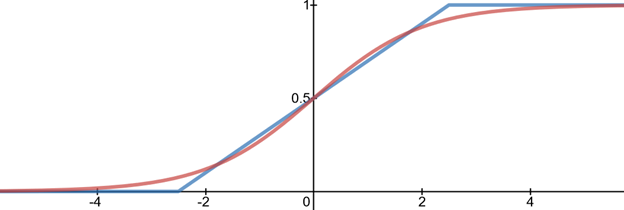
\includegraphics[width=\linewidth]{\picPath/quant_1.png}
  \caption{Hard Sigmoid}
  \label{fig:quant_1}
  \end{center}
\end{figure}

То есть мы заменяем функцию активации на более простую, которая использует только операции сложения, деления и умножения. Точно так же делаем с тангенсом. В итоге получая, что кроме сравнения чисел и умножения их между собой у нас нет других операций. В таблице 3.2 представлены примеры таких функций
\begin{table}[H]
% Подпись таблицы
\caption{Сгрубленные функции}
% Ссылка на таблицу
\label{table_1}
\begin{tabularx}{\textwidth}{|X|X|} % Столько X, сколько столбцов
\hline
Оригинальная активация & Сгрубленный аналог \\ \hline
$$\sigma (x)=\frac{1}{1+\exp{-x}}$$ & $$\sigma_{hard}(x)=\begin{Bmatrix} 0 & x \leq -3\\ 1 & x \geq 3\\ \frac{x}{6}+\frac{1}{2} & otherwise \end{Bmatrix}$$ \\
$$Tanh(x)=tanh(x)$$ & $$Tanh_{hard}(x)=\begin{Bmatrix} -1 & x < -1\\ 1 & x > 1\\ x & otherwise \end{Bmatrix}$$ \\ \hline
\end{tabularx}
\end{table}

С активациями остается еще одна небольшая проблема. Сами их значения могут быть произвольными. Пример: мы подаем на вход два числа 100, -5, и получаем на выходе какого-то слоя -1310. При этом, в эту же сеть подаем другие значения, например, -7, 12, и получаем всего 115. Таким образом, значение после применения активации определяется тем, какие входные данные будут поданы на сеть. Таким образом, нужно еще отдельно подумать, как для значений после активации посчитать эти параметры — растяжение и смещение. Для этого есть несколько подходов:
\begin{itemize}
    \item динамическая квантизация
    \item статическая квантизацияя
    \item квантизация во время тренировки
\end{itemize}

\section{Динамическая квантизация}

Для динамической квантизации применяют следующий алгоритм: мы берем какой-то слой, для него считаем все взвешенные суммы и перед тем, как пропустить матрицы сквантованных значений через активацию, мы прямо на лету переводим все элементы обратно во FLOAT32 и для этих FLOAT32 применяем функцию активации, получаем все исходные значения.  Таким образом, мы получаем набор чисел, которые составляют диапазон на текущем слое. Для них, прямо во время вычисления, мы подсчитывает эти параметры S и Z для смещения и растяжения, и исходя из этих значений квантуем наши активации, которые после этого передаем дальше по сети.

Следует отметить, что существует два типа квантизации для функций активаций. Симметричный и ассиметричный. Их различие состоит в том, что для симметричного способа квантизации параметр смещения равен нулю, тогда как для ассимитричной этот параметр вычисляется описанными выше способами. На рисунке 3.2 схематично представлено динамическое квантование

\begin{figure}[H]
\begin{center}
  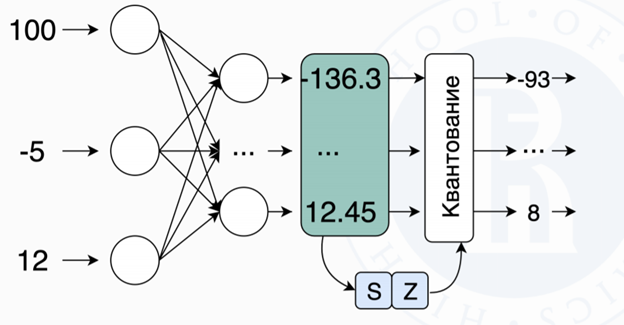
\includegraphics[width=\linewidth]{\picPath/quant_2.png}
  \caption{Динамическое квантование}
  \label{fig:quant_2}
  \end{center}
\end{figure}

\section{Статическая квантизация}
Альтернативный прием — это прием статической квантизации. Статическое квантование после обучения включает в себя не только преобразование весов из float в int, как при динамическом квантовании, но также выполнение дополнительного шага первой подачи пакетов данных через сеть и вычисления результирующих распределений различных активаций (в частности, это выполняется путем вставки модулей наблюдателя в разные точки, которые записывают эти данные). Эти распределения затем используются для определения того, как конкретно различные активации должны быть квантованы во время вывода. После этого, мы зафиксируем эти два значения( scale и zero-point), и уже будем всегда одинаково квантовать все активации в нашей нейронной сети, ожидая, что те данные, которые будут нам подавать на вход, в последующем будут из того же распределения, что и изначальные данные из обучающие выборки. На рисунке 3.3 схематично представлено динамическое квантование

\begin{figure}[H]
\begin{center}
  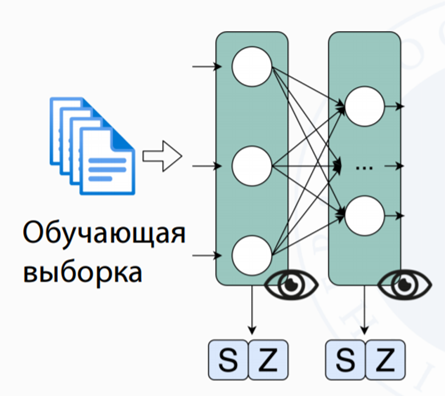
\includegraphics[width=\linewidth]{\picPath/quant_3.png}
  \caption{Статическое квантование}
  \label{fig:quant_3}
  \end{center}
\end{figure}

Важно отметить, что этот дополнительный шаг позволяет нам передавать квантованные значения между операциями вместо преобразования этих значений в числа с плавающей запятой - а затем обратно в целые числа - между каждой операцией, что приводит к значительному ускорению. 

\section{Бинаризация}
"Плюс-минус" квантование было предложено еще в 1990 году. Этот метод уменьшает все веса до 1-битных представлений, удаляя все дорогостоящие умножения. Бинаризованные нейронные сети (BNN) имеют только 1-битные веса и часто 1-битные активации. 0 и 1 кодируются для представления -1 и +1 соответственно. В двоичной арифметике однобитовые операции могут выполняться с использованием $AND$, $XNOR$ и $bitcoin$. Как было показано выше свертки можно разложить в произведение матриц, а это набор операций умножения и сложения.

Одноразрядные скалярные произведения вычисляются, как показано в уравнении 3.8, где $AND$ является побитовой операцией И, а $bitcoin$ подсчитывает число единиц в битовой строке. Это расширяется в многобитовые операции, как показано в уравнении 3.9
\begin{equation}
    x \cdot y = bitcoin(and(x,y)), \forall i,x_i,y_i \in \left \{ 0,1 \right \}
\end{equation}

\begin{equation}
    x \cdot y = \sum_{m=0}^{M-1}\sum_{k=0}^{K-1}2^{m+k}bitcoin[and(c_m(x),(c_m(y))], c_m(x)_i, c_k(y)_i \in \left \{ 0,1 \right \}\forall i,m,k
\end{equation}
Где $X$, $Y$, $M$-bit и $K$-bit целые числа с фиксированной запятой.\\
$c_m(x)$, $c_m(y)$ - битовые вектора

Удалив сложные операции умножения с плавающей запятой, сети значительно упрощаются с помощью простого накопительного оборудования. Бинаризация не только уменьшает размер сети до 32 раз, но также резко снижает использование памяти, что приводит к значительному снижению затрат на ресурсы. Однако сокращение 32-битных параметров до одного бита приводит к значительной потере информации, что снижает точность прогнозирования. Большинство квантованных двоичных сетей значительно уступают 32-битным конкурентам.

Существует два основных метода сокращения значений с плавающей запятой до одного бита:
\begin{itemize}
    \item стохастический
    \item детерминированный
\end{itemize}

Стохастические методы рассматривают глобальную статистику по значениям входных данных, чтобы определить вероятность того, что какой-либо параметр будет равен -1 или +1. Детерминированная бинаризация напрямую вычисляет битовое значение на основе порога, обычно в качестве порога выступает 0, что приводит к сигнум функции. Детерминированную бинаризацию гораздо проще реализовать аппаратно.

Был предложен один из методов бинаризации, двоичное соединение (BC), оно представляет собой ранний стохастический подход к бинаризации нейронных сетей. Авторы преобразовали веса в двоичную форму как для прямого, так и для обратного распространения. Уравнение 3.10 показывает принятую стохастическую бинаризацию посредством сгрубленного сигмоида. И активации, и градиенты используют числа с 32-битной плавающей запятой. Обученные сети BC показали ошибку классификации 1,18\% на MNIST датасете и 8,27\% на CIFAR-10.
\begin{equation}
    x^b=\left\{\begin{matrix}
    +1 & p=\sigma(x)\\ 
    -1 &  1-p
\end{matrix}\right.
\end{equation}
Немного позже был предложен способ бинаризовать и активации. Авторы также предложили ядро для двоичного умножения матрица на ГПУ, которое ускорило вычисления в 7 раз. Учитывая стоимость вычислений для стохастической бинаризации, они пошли на компромисс, применив детерминированную бинаризацию в большинстве случаев. 

Такая сеть показывает ошибку в 0,86\% для MNIST, 2,53\% для SVHN и 10,15\% для CIFAR-10. Результаты точности на наборе данных ImageNet для бинаризованных AlexNet и GoogleNet составляют 36,1\% и 47,1\% соответственно, в то время как исходные сети FP32 достигают 57\% и 68\% соответственно.

\section{Квантизация во время тренировки}
Последний прием, который нужно рассмотреть — это квантизация в процессе обучения. 
Можно заметить, что так как нейронная сеть большая, и мы квантуем очень много чисел, мы можем потерять довольно много информации, и ошибка таким вот образом накопится поверх всей сети. Для того чтобы избежать этого, мы можем пытаться обучать нейронную сеть вместе с процессом квантования. По сути, данный прием работает интуитивно понятно, после каждого шага градиентного спуска, мы берем и квантуем сразу же все веса.

Таким образом, после того, как мы посчитаем все эти значения, следующий шаг градиентного спуска, будет считаться уже из новых уже квантованных весов. Таким образом, у модели получится вычислить более оптимальные параметры для текущего квантованного состояния.

Мы сделали градиентный шаг и куда-то образно попали по направлению минимума, и после этого сразу сгрубили наше значение квантованием. Таким образом, уже следующий шаг градиентного спуска будет считать свое значение не из той эфемерной точки, а из новой, конкретной, которая появилась после квантования. На рисунке 3.4 изображен процесс оптимизации.

\begin{figure}[H]
\begin{center}
  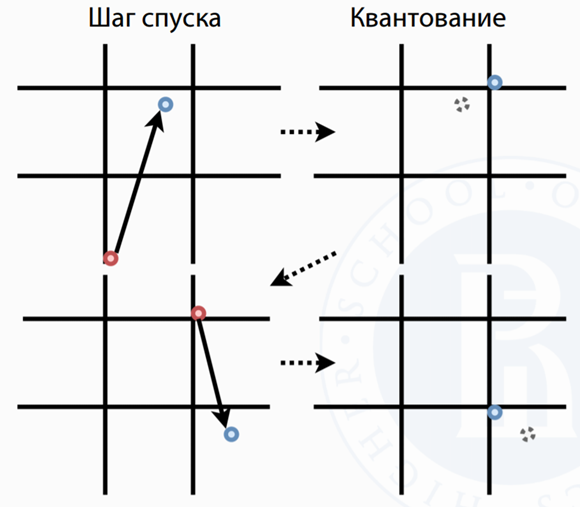
\includegraphics[width=\linewidth]{\picPath/quant_4.png}
  \caption{Процесс оптимизации при квантизации во время тренировки}
  \label{fig:quant_4}
  \end{center}
\end{figure}

Таким образом, мы надеемся, что сеть сможет как-то компенсировать эти потери от квантования в процессе обучения.

Отдельно стоит отметить, что сам градиент будет считаться FLOAT32 по той причине, что нам все таки требуется быстрая сходимость. Однако, сами веса можем квантовать после каждого шага. 

Обучение с низкой числовой точностью включает использование значений с низкой точностью как для прямого, так и для обратного распространения при сохранении накопленных результатов с полной точностью. В обучении со смешанной точностью используется FP16 или 16-битное целое число (INT16) для значений весов. Было показано, что такой точности не хватает для значений градиента. Как показано на рисунке 3.5, веса с полной точностью поддерживаются для обновления градиента, в то время как все остальные операнды используют числа с FP16.
\begin{figure}[H]
\begin{center}
  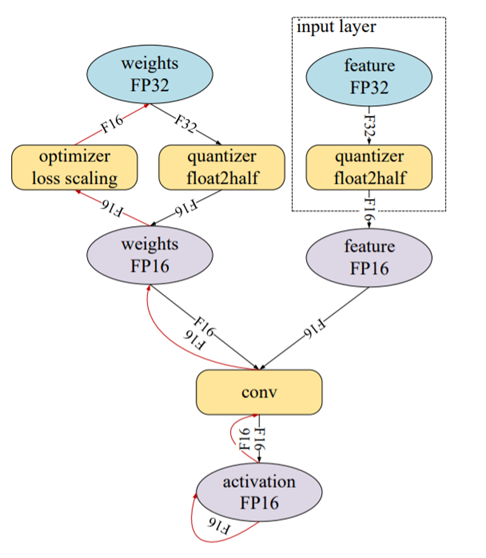
\includegraphics[width=\linewidth]{\picPath/quant_5.png}
  \caption{Mixed precision training}
  \label{fig:quant_5}
  \end{center}
\end{figure}

Метод масштабирования потерь (loss scaling) применяется для предотвращения влияния очень малых градиентов величины на процесс обучения, поскольку любое значение меньше $2 ^ -24$ становится нулевым с половинной точностью (FP16). В частности, некоторый масштабируемый оператор вводится в значение потерь перед обратным распространением. Как правило, средство масштабирования представляет собой оптимальное значение сдвига битов двойки, полученное эмпирически или с помощью статистической информации.

Для бинаризованной сети, которая имеет двоичные значения весов, неэффективно обновлять веса с использованием методов градиентного спуска из-за очень малых производных. На ранних стадиях исследований сети с квантованием обучались с помощью варианта байесовского инференса, называемого ожиданием обратного распространения (expectation back propagation, EBP). Этот метод назначает ограниченную точность параметров (например, бинаризованную) весов и активаций. 

EBP инферит сети с квантованными весами, обновляя апостериорные распределения по весам. Апостериорные распределения обновляются путем дифференцирования параметров обратного распространения ошибки. Метод BinaryConnect (BC) принял вероятностную идею EBP, но вместо оптимизации апостериорного распределения весов BC сохранил веса с плавающей запятой для обновлений, а затем квантовал их в двоичные значения. Реальные веса обновляются с использованием ошибки обратного распространения, просто игнорируя бинаризацию в обновлении. 

Бинаризованная сеть имеет только 1-битные параметры - ± 1, квантованные от кусочно постоянной функции сигнум (sign function). Однобитовые параметры недифференцируемы, поэтому невозможно вычислить градиенты, необходимые для обновления параметров. Было показано, что для эффективности алгоритмов SGD требуется от 6 до 8 битов. Чтобы обойти эти ограничения, straight-through estimator (STE) метод был применен для распространения градиентов с использованием дискретизации. Уравнение 3.11 показывает STE для бинаризации.

\begin{equation}
\begin{split}
    Forward: w_b = sign(w_r)\\
    Backward: \frac{\partial c}{\partial w_r}=\frac{\partial c}{\partial w_b}, \left | w_r \right | \leq1
\end{split}
\end{equation}
Где $c$ - целевая функция\\ 
$w_r$- действительные веса\\
$w_b$ - бинаризованные вес, полученные сигнумом.

Таким образом, STE обходит функцию бинаризации чтобы напрямую вычислить градиент со значениями FP32. Затем веса с плавающей запятой обновляются с использованием таких методов, как SGD. Очень похоже на метод, который используется для квантования в целые числа или при тренировке со смешанной точностью. Во избежание приближения действительных весов к бесконечности, в бинаризированных сетях обычно ограничивают веса с плавающей запятой в желаемом диапазоне ± 1.

Позднее Alpha-Blending (AB) был предложен в качестве замены STE. Поскольку STE напрямую устанавливает градиенты функции квантования в единицу, как можно видеть в уравнении 3.11, то была высказана гипотеза, что сети с STE могут нести потери в точности. На рисунке 3.6 показано, что AB вводит дополнительный масштабный коэффициент $\alpha$. Сохраняются как действительные, так и квантованные веса. Во время обучения $\alpha$ постепенно увеличивается до 1, пока не будет получена полностью квантованная сеть.
\begin{figure}[H]
\begin{center}
  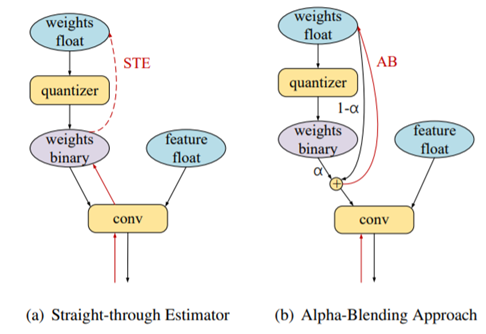
\includegraphics[width=0.7\linewidth]{\picPath/quant_6.png}
  \caption{Alpha-Blending}
  \label{fig:quant_6}
 \end{center}
\end{figure}

Подводя итог, квантизация — класс методов, которые могут значительно уменьшить размер нейронной сети и ускорить ее вычисление. 

В таблице 3.3 можно видеть, что квантование, на большинстве популярных архитектур нейронных сетей, дает очень хорошие результаты. Ускорение позволяет некоторым сетям работать до трех раз быстрее, при этом сама точность не очень падает, а в некоторых случаях, удивительным образом, даже возрастает. 

\begin{table}[H]
% Подпись таблицы
\caption{Результаты квантизации популярных архитектур}
% Ссылка на таблицу
\label{table_1}
\begin{tabularx}{\textwidth}{|X|X|X|X|} % Столько X, сколько столбцов
\hline
Модель & Ускорение & Оригинальная точность, \% & Точность после квантизации,\% \\ \hline
googlenet & x2.7 & 73.45 & 73.25 \\
mobilenet_v2 & x2.6 & 72.40 & 73.15\\ 
resnet18 & x1.6 & 70.00 & 69.45\\ 
resnet50 & x2.7 & 76.95 & 76.60\\ \hline

\end{tabularx}
\end{table}

\section{Программная реализация квантизации нейронной сети}
В качестве нейронной сети возьмем такую же сеть, которую мы использовали в главе 2, ResNet18. Датасет также остался тем же, FashionMNIST. Весь код представлен в приложении В.

\subsection{Статическая квантизация}
Статическая квантизация позволяет сразу все операции перевести в int, без необходимости дополнительно что-то расчитывать в процессе предсказания.

По сравнению с моделью из главы про разряжение нейронной сети, архитектура повлекла небольшие изменения. В частности, так как квантизация не происходит динамически, необходимо дополнительно руками квантовать входные данные и деквантовать ответ. Это можно видеть в $forward$ методе класса $ResNet18$.

Также стоит обратить внимание на применение $nn.quantized.FloatFunctional()$ при выполнении $skip connection$ в ResNet архитектуре. Это необходимо для правильного выполнения операции сложения со сквантованным входом и весами в представлении float32. 

Статическое квантование после обучения включает в себя не только преобразование весов из float32 в int, как при динамическом квантовании, но также выполнение дополнительного шага первоначальной прогонки выборки обучающих данных через сеть и вычисления результирующих распределений различных активаций (в частности, это выполняется путем вставки модулей, так называемого наблюдателя, в нужные места после каждой операции, которые записывают эти данные). Эти распределения затем используются для определения того, как конкретно различные активации должны быть сквантованы во время вывода (вычисляется свой коэффициент масштабирования и смещения). Важно отметить, что этот дополнительный шаг позволяет нам передавать квантованные значения между операциями вместо преобразования этих значений в числа с плавающей запятой - а затем обратно в целые числа - между каждой операцией, что приводит к значительному ускорению.

После обучения полученное качество составляет 92.5\% на валидационной выборке. Это будет нашим базовым уровенем. Далее замерим время инференса сети на ЦПУ. Чтобы замер был честный, отключим возможность PyTorch использовать несколько потоков и будем использовать всего один поток вычислений. Как видно в приложении В, скорость инференса сети в среднем 6 минут и 31 секунда. Измерим вес сети, занимаемой памяти в хранилище данных. Она составляет примерно 44 мб памяти. Теперь применим алгоритмы квантизации и попробуем уменьшить это значение в несколько раз, при этом не потеряв сильно в качестве.

Для моделей мы также можем указать конфигурационный файл квантования, где в частности можно указать библиотеку для работы с квантованными значениями. Далее устанавливаем модули подсчета параметров квантования. По умолчанию исползуется $HistogramObserver$, это модуль, который рассчтывает параметры на основе гистрограммы распределения значнеий для конкретного слоя.

Прогоняем всю обучающую выборку через сеть. Само значение нам не интересно, нам важно, чтобы посчитались параметры. Фиксируем полученные веса и параметры квантизации. 

Применяя алгоритм квантизации, удалось сжать ее размер примерно в 4 раза. Теперь вместо 44 мб. она занимает всего 11 мб. В приложении В можно видеть, что теперь все веса имеют свой коэффициент масштабирования и смещения, а также  int8 представление на примере линейного слоя. По результатам тестирования можно сделать вывод, что просадки в точности сети нет, покрайней мере на наших тестовых данных удалось достичь метрики оригинальной модели. Время инференса составляет 3 минуты и 52 секунды в среднем, что почти в два раза меньше, чем было.

\subsection{Квантизация в процессе обучения}
Этот метод заключается в том, что квантование происходит на каждом шаге градиентного спуска. С QAT (Quantization-aware training) все веса и активации «поддельно квантуются» во время как прямого, так и обратного проходов обучения: то есть числа с плавающей точкой округляются до имитации значений int8, но все вычисления по-прежнему выполняются во float32 представлении. Таким образом, все корректировки веса во время обучения производятся с учетом того факта, что модель в конечном итоге будет квантована; поэтому после квантования этот метод обычно дает более высокую точность, чем динамическое квантование или статическое квантование после обучения.

Общий рабочий процесс для фактического выполнения QAT очень похож на предыдущий. Мы можем использовать ту же модель, что и раньше: для обучения с учетом квантования не требуется дополнительной подготовки. Нам нужно только использовать $qconfig$, указывающий, какой тип фальшивого квантования должен быть вставлен после весов и активаций, вместо указания модулей наблюдателей (Histogram observers), как было раньше.

Добавляем конфигурацию, после чего подготавливаем модель для обучения с квантованием. Модель внутри себя автоматически будет обновлять веса с учетом квантования. После обучения с квантованием, фиксируем квантованные веса и параметры. Таким образом получаем финальную сеть для последующего использования. В таблице 3.4 представлена сводная таблица результатов квантизации.

\begin{table}[H]
% Подпись таблицы
\caption{Результаты алгоритмов квантизации}
% Ссылка на таблицу
\label{table_3.1}
\begin{tabularx}{\textwidth}{|X|X|X|X|} % Столько X, сколько столбцов
\hline
Алгоритм & Точность, \% & Размер сети, мб & Время инференса, сек\\ \hline
baseline & 92.5 & 44 & 391\\ \hline 
static quantization &  92.5 & 11 & 232\\ \hline 
QAT & 92.5 & 11 & 232\\ \hline 
\end{tabularx}
\end{table}

\chapter{Фреймворки для компрессии нейронных сетей}
Большинство сетей были разработаны для достижения максимально возможной точности для конкретно поставленной задачи без учета времени выполнения вычислений и способах развертывания подобных сетей на реальных устройствах клиента. При развертывании модели руководящим принципом является компромисс между производительностью и точностью. Это наблюдение побудило к разработке методов обучения более эффективных с вычислительной точки зрения моделей глубокого обучения (DL), чтобы эти модели можно было использовать в реальных приложениях с ограниченными ресурсами, например, на различного рода мобильных устройствах. 

В предыдущих главах курсовой работы были рассмотрены основные методы, позволяющие оптимизировать модели глубокого обучения для их ускорения, эффективного сжатия и при этом не теряя сильно в итоговом качестве на поставленной задаче. Одно из наиболее интересных направлений – это алгоритмы квантизации, спарсификации и отсечения. Мы уже рассмотрели теоритическую составляющую данных инструментов и посмотрели на простых практических примерах, как можно реализовать данные алгоритмы и применить их в своих исследовательских проектах. В этой же главе мы рассмотрим какие существуют фреймворки для этих целей и как мы можем внедрить такие инструменты в сложный проект промышленного машинного обучения, который будет использоваться другими людьми для решения своих задач. 

Для начала мы постараемся ответить,  а зачем нам для этого иметь фреймворк. Фреймворк – это программная платформа, которая объединяет программное обеспечение, различные инструменты для какого-то большого программного проекта. Конечно, в теории мы можем каждый раз реализовывать все представленные алгоритмы компрессии под конкретную нашу текущую задачу или пользоваться какими-то отдельно предлагаемыми компонентами. Но это будет неэффективно с точки зрения затрат труда программистов, переиспользования кода,  а также это будет иметь ограниченную функциональность и скорее всего ограниченную масштабируемость.

В настоящее время прилагаются многочисленные усилия по внедрению алгоритмов сжатия не только в исследовательское сообщество, но и для более широкого круга пользователей, заинтересованных в реальных приложениях глубокого обучения. Почти все современные фреймворки по глубокому обучению так или иначе поддерживают функции компресии. В предыдущих главах мы уже видели, как применять инструменты библиотеки PyTorch для оптимизации сети ResNet. На данный момент инструменты этой библиотеки еще только развиваются. 
Квантование модели до точности INT8 в настоящее время становится основным подходом для ускорения вывода с минимальными усилиями. Одна из влиятельных работ в этой области, в которой представлено  квантование во время обучения (QAT) для TensorFlow. В этой работе освещаются проблемы алгоритмических аспектов равномерного квантования для CNN с последующей дотренировкой, а также предлагается эффективный пайплайн, предназначеный для конкретного оборудования. QAT основан на операции ложного квантования, которая, в свою очередь, может быть представлена парой операций квантования / деквантования. Важной особенностью предлагаемого программного решения является автоматическая вставка операций ложного квантования, что упрощает оптимизацию модели для пользователя. Однако у этого подхода есть существенные недостатки, а именно увеличенное время обучения и потребление памяти. Другая проблема заключается в том, что метод квантования основан на наивном подходе min / max и потенциально может достичь худших результатов, чем более сложные стратегии выбора диапазона квантования. 

Другой фреймворк Graffitist на основе TensorFlow, который также использует квантование при обучении, данный фреймворк направлен на улучшение методов QAT, обеспечивая балансировку, уточнение результирующих параметров квантования для каждого тензора, посредством обучения этих параметров вместе с весами сети. У этой схемы есть недостаток, она ограничена симметричным квантованием и допускает только ширину квантования 4/8 бит, в то время как этого не всегда достаточно и как минимум исследования показывают, что для архитектуры MobileNetV3 ассиметричная квантизация критически важная для получения хороших результатов. Кроме того, данное решение подразумевает дополнительные преобразования графа во время процесса квантования, таких как свертывание операции пакетной нормализации, они требуют дополнительные вычисления. 

Из инструментов для сжатия моделей на основе фреймворка PyTorch, помимо стандартных инструментов, предлагаемых авторами библиотеки, существует популярный фреймворк Neural Network Distiller. Он содержит реализацию алгоритмов различных методов сжатия, таких как квантование, бинаризация, отсечение фильтров и другие. Однако это решение в основном ориентировано на исследовательские задачи, а не на применение методов в реальных задачах использования. Кроме того, весь широкий спектр алгоритмов, предлагаемый этим фреймворком доступен только для задачи классификации, тогда как, например, для задачи детектирования объектов представлены лишь алгоритмы спарсификации. Наиболее важным недостатком Distiller является отсутствие готового к использованию пайплайна от сжатия модели до ее развертывания на целевом оборудовании клиента.

Не так давно, в 2020 году появился новый фреймворк, NNCF (Neural Network Compression Framework) который способен решить выше описанные проблемы. Он использует последние достижения различных методов сжатия сети и реализует некоторые из них, а именно квантование, разреженность, отсечение фильтров и бинаризацию. Эти методы позволяют создавать более удобные для оборудования модели, которые можно эффективно запускать на аппаратных вычислительных модулях общего назначения (ЦП, ГП) или на специализированных ускорителях глубокого обучения. Реализованные методы и их комбинации могут быть успешно применены к широкому кругу архитектур и задач для ускорения вывода при сохранении точности исходной модели. Главное преимущество это то, что данный фреймворк можно использовать как отдельный пакет, который можно легко интегрировать в существующий обучающий код с минимальной адаптацией.

В целом структура NNCF включает в себя следующие важные особенности и возможности:
\begin{itemize}
    \item Поддержка алгоритмов квантования, бинаризации, разреженности и отсечения фильтров с дотренировкой (QAT и итеративный прунинг).
    \item Автоматическое преобразование динамического графа модели в PyTorch - модель оборачивается в некоторую обертку, и в граф модели вставляются дополнительные слои, необходимые для процесса квантования и прунинга.
    \item Возможность объединять различные методы сжатия и применять несколько из них одновременно.
    \item В фреймворке представлены обучающие примеры для задач классификации изображений, обнаружения объектов и семантической сегментации, а также файлы конфигурации для сжатия ряда популярных архитектур.
    \item Возможность интегрировать обучение с применением сжатия в сторонние репозитории с минимальными модификациями существующих пайплайнов обучения, что позволяет интегрировать NNCF в крупномасштабные репозитории
    \item Слои с аппаратным ускорением для быстрой дотренировки модели и для поддержки обучения с использованием нескольких графических процессоров.
    \item Совместимость с OpenVINO Toolkit для эффективного инференса модели.
\end{itemize}

Также сейчас NNCF развивается в направлении поддержки моделей на TensorFlow. Таким образом, данный фреймворк можно назвать универсальным решением для внедрения алгоритмов сжатия для промышленного машинного обучения.

Для достижения целей сжатия во время обучения, NNCF оборачивает обычный базовый объект модели PyTorch с точность FP32 в оболочку NNCFNetwork. Каждый метод сжатия воздействует на эту оболочку, определяя следующие основные компоненты:
\begin{itemize}
    \item Построитель алгоритмов сжатия (Compression Algorithm Builder) - объект, определяющий изменения, которые необходимо внести в базовую модель, чтобы имитировать сжатие, характерное для текущего алгоритма.
    \item Контроллер алгоритма сжатия (Compression Algorithm Controller) - объект, который обеспечивает доступ к параметрам алгоритма сжатия и статистике во время обучения (например, точная разрядность квантования определенного слоя в модели или уровень разреженности в определенном слое).
    \item Потери при сжатии, представляющие дополнительную функцию потерь, введенную в алгоритм сжатия для его облегчения.
    \item Планировщик сжатия (Compression Scheduler), который может быть определен для автоматического управления параметрами метода во время процесса обучения, с обновлениями для каждого батча или эпохи без явного использования контроллера алгоритма сжатия.
\end{itemize}

Авторы постулируют, что потенциально любой метод сжатия может быть реализован с использованием выше описанных абстракций. Например, метод разреженности на основе регуляризации (RB), реализованный в NNCF, вводит оценки важности для весов сверточных и полносвязных слоев, которые являются дополнительными обучаемыми параметрами. 

Двоичная маска весов, основанная на пороговой оценки важности, добавляется специализацией объекта Compression Algorithm Builder, действующего на объект NNCFNetwork, модифицируя его таким образом, что во время прямого прохода по сети веса умножаются на маску перед выполнением самой операции. Чтобы эффективно обучать эти дополнительные параметры, метод RB спарсификации определяет LASSO регуляризацию, которая должна быть минимизирована вместе с функцией потери основной задачи, а также указывает планировщик для постепенного увеличения скорости разреженности после каждой эпохи обучения. Про LASSO регуляризаю и данный метод более подробно было описано в главе 3.

Как упоминалось ранее, одной из важных функций фреймворка является автоматическое преобразование модели, то есть вставка вспомогательных слоев и операций, необходимых для конкретного алгоритма сжатия. Для этого требуется доступ к динамическому графу модели, который фактически недоступен в среде PyTorch. Чтобы решить эту проблему, они изменяют операции модуля PyTorch и обертывают базовые операторы, такие как $torch.nn.functional.conv2d$, чтобы иметь возможность отслеживать их вызовы во время инференса модели и выполнять код включения сжатия до и / или после вызовов этих операторов.

Еще одним важным нововведением NNCF является поддержка объединения алгоритмов, при которой пользователи могут создавать собственные конвейеры сжатия, комбинируя несколько методов в один пайплайн. Примером этого являются модели, которые могут быть разреженными и в то же время квантованными. Функция объединения, реализованная внутри фреймворка, не требует каких-либо доработок со стороны пользователя. Чтобы применить это, нужно всего лишь указать набор методов сжатия, которые будут применяться в файле конфигурации. На рисунке 4.1 показан общий пайплайн для сжатия моделей. 

\begin{figure}[H]
\begin{center}
  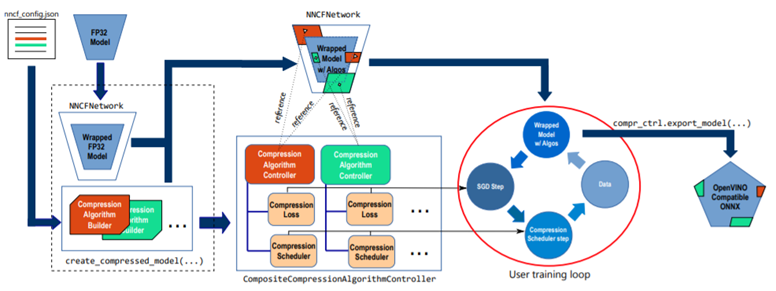
\includegraphics[width=\linewidth]{\picPath/nncf_1.png}
  \caption{NNCF pipeline}
  \label{fig:nncf_1}
 \end{center}
\end{figure}

На начальном этапе модель оборачивается оболочкой NNCFNetwork, которая сохраняет исходную функциональность объекта модели неизменной, чтобы его можно было в дальнейшем использовать в процессе обучения, как если бы он вообще не был изменен.

Затем создается один или несколько конкретных алгоритмов сжатия, которые применяются к обернутой модели. На этом этапе создается один или несколько контроллеров алгоритмов сжатия (по одному для каждого алгоритма), а также окончательный объект модели с необходимыми настройками, связанными со сжатием. Затем обернутую модель можно дообучить на целевом наборе данных, используя либо исходный обучающий пайплайн, либо слегка измененный на случай, если пользователь решил применить алгоритм, учитывающий
дополнительные потери после прунинга и/или квантизации, которые необходимо минимизировать.

Ниже приведен пример того, как можно использовать фреймворк в самом простом случае:

\lstset{language=Python}
\begin{lstlisting}
import torch
import nncf
from nncf (mport create_compressed_model, NNCFConfig, 
        register_default_init_arg)
\end{lstlisting}

Подготавливаем модель:
\begin{lstlisting}
from torchvision.models.resnet import resnet50
model = resnet50()
\end{lstlisting}

Загружаем конфиг, требуемый для определния основных параметров сжатия:
\begin{lstlisting}
nncf_config = NNCFConfig.from_json("resnet50_int8.json")
\end{lstlisting}

Предоставляем загрузчиков данных, если требуется для алгоритма:
\begin{lstlisting}
nncf_config = register_default_init_args(nncf_config, 
                                        train_loader, 
                                        loss_criterion)
\end{lstlisting}

Применяем желаемый алгоритм к модели:
\begin{lstlisting}
comp_ctrl, compressed_model = create_compressed_model(
                                            model, 
                                            nncf_config)
\end{lstlisting}

Далее дооубачем нашу модель, как обчно, используя свой тренировочный пайплайн. После этого мы можем экспортировать готовую модель в ONNX и затем сконвертировать в IR представление для инференса через средства OpenVINO toolkit:
\begin{lstlisting}
comp_ctrl.export_model("compressed_model.onnx")
torch.save(compressed_model.state_dict(), 
           "compressed_model.pth")
\end{lstlisting}

В таблице 4.1 указана сводная информация об моделях, которые можно получить, применяя данный фрейморк. Ссылка на официальный репозиторий : $https://github.com/openvinotoolkit/nncf$

\begin{table}[H]
% Подпись таблицы
\caption{Результаты сжатия нейронных сетей посредством фреймоврка NNCF}
% Ссылка на таблицу
\label{table_2}
\begin{tabularx}{\textwidth}{|X|X|X|X|} % Столько X, сколько столбцов
\hline
Модель & алгоритм & FP32 & после компрессии \\ \hline
ResNet-50 & 44.8\% INT8 / 55.2\% INT4  & 76.16 & 76.2 \\ \hline
Inception V3 & INT8 + Sparsity 61\% (RB)  & 77.34 & 77.58 \\ \hline
MobileNet V2 & 46.6\% INT8, 53.4\% INT4  & 71.93 & 70.92 \\ \hline 
SqueezeNet V1.1 & Mixed, 54.7\% INT8 / 45.3\% INT4  & 58.24 & 58.9 \\ \hline
ResNet-34 & Filter pruning, 40\%, geometric median criterion  & 73.3 & 72.73 \\ \hline
GoogLeNet & Filter pruning, 40\%, geometric median criterion  & 69.75 & 68.82 \\ \hline
\end{tabularx}
\end{table}

Таким образом, авторы фреймворка уделяют особое внимание юзабилити для пользователей и упрощают настройку процесса сжатия, а также была произведена апробация фреймворка на широком спектре моделей и задач. Модели, полученные с помощью NNCF, демонстрируют отличные результаты с точки зрения соотношения точности и производительности. 

\chapter{Сжатие нейронной сети для проекта RGB антиспуфинга}
Spoof в целом означает подделку, fake, в данном случае face anti-spoofing это попытка обмануть системы по распознованию лиц различными способами. Алгоритм антиспуфинга лиц позволяет определить, является ли лицо, снятое системой распознования лиц, настоящим или поддельным. RGB антиспуфинг - это подкласс задачи, в которой используется лишь одна модальность, RGB изображение без карт глубины или инфокрасных датчиков.

В качестве бэкбона алгоритма выбрана MobileNetV3. Основные цели проекта состояли в легковесности сети, максимальной производительности на мобильных устройствах, при этом, качество модели не должно было бы сильно уступать state of the art аналогу, сети AENet. Конечная модель вошла в релиз публичных моделей OMZ OpenVINO 2020Q4. В качестве датасета был использован датасет CELEBA-SPOOF. В сухом остатке, данную задачу можно рассматривать как задачу бинарной классификации по определению двух классов spoof/real. 

В данной курсовой работе мы попробуем применить фреймворк NNCF для сжатия данной нейронной сети и получения еще большего выигрыша в скорости работы. 

Был выбран алгоритм асинхронной квантизации в int-8. Ниже представлена выжимка конфигурационного фаила nncf, подготовленного в расширении $.json$:

\begin{lstlisting}
 "nncf_config": {
            "compression": [
            {
                "algorithm": "quantization",
                "initializer": {
                    "range": {
                        "num_init_samples": 8192
                    },
                    "batchnorm_adaptation": {
                        "num_bn_adaptation_samples": 8192
                    }
                }
            }
        ]
    }
\end{lstlisting}

где $num\_init\_samples$ означает количество выборок из обучающего набора данных для использования в качестве входных данных модели для целей установки начального минимального и максимального диапазонов квантования \\
$num\_bn\_adaptation\_samples$ - Количество выборок из обучающего набора данных, которые должны пройти через модель при инициализации, чтобы обновить статистику пакетной нормализации исходной модели. Фактическое количество образцов будет кратным размеру батча.

Далее в классах построения датасета CELEBA-SPOOF мы регистрируем загрузчик тренировочных данных  с помощью $register\_default\_init\_args$. В функции построения моделей мы добавляем регистрацию компрессированной модели с помощью $create\_compressed\_model$. Обернутая модель передается в пайплайн тренировки. 

В процессе тренировки мы будем следить за компрессионными стадиями. Сначала зададим, что лучшая стадия компресии это изначальная fp32 модель. $best\_compression\_stage = CompressionStage.UNCOMPRESSED$. Будем запомнать лучшую метрику точности, учитывая ступень компрессии. Это означает, что если текущая точности меньше, чем лучшая, то контрольная точка все равно может быть лучше, если текущая стадия сжатия больше, чем лучшая. Этапы сжатия рассматриваются в порядке возрастания: $UNCOMPRESSED$, $PARTIALLY\_COMPRESSED$, $FULLY\_COMPRESSED.$

После этого будем сохранять лучшую контрольную точку:

\lstset{language=Python}
\begin{lstlisting}
is_best_by_accuracy = (acc1 > best_acc1 and 
           compression_stage == best_compression_stage)
is_best = (is_best_by_accuracy or 
            compression_stage > best_compression_stage)
if is_best:
    best_acc1 = acc1
best_compression_stage = max(compression_stage, 
                                best_compression_stage)
\end{lstlisting}

В конце тренировки мы можем экспортировать полученную int-8 модель в ONNX с последующей конверсией в OpenVINO представление.

В таблице 5.1 представлены результаты примененного алгоритма в сравнении с FP32 моделью. Производительность была замерена с помощью OpenVINO Deep Learning Benchmark на процессоре Intel Xeon Gold 6230. В качестве метрики производительности было выбрано FPS (frame per second)

\begin{table}[H]
% Подпись таблицы
\caption{Результаты сжатия MobileNetV3 посредством фреймоврка NNCF}
% Ссылка на таблицу
\label{table_4.1}
\begin{tabularx}{\textwidth}{|X|X|X|X|X|X|X|} % Столько X, сколько столбцов
\hline
Модель & Accuracy FP32 & AUC FP32 &  FPS FP32 & Accuracy INT8 & AUC FP32 &  FPS FP32 \\ \hline
MNV3 Spoof large & 94.9\% & 0.998 &  2668.57 & 94.76\% & 0.997 & 4238.66 \\ \hline
MNV3 Spoof small & 93.5\% & 0.994 &  6219.94 & 93.34\% & 0.994 & 7659.16 \\ \hline
\end{tabularx}
\end{table}

По результатам видно, что удалось удачно интегрировать NNCF фреймворк в проект антиспуфинга, ускорить работу моделей примерно в 1.5 раза, при этом просадка в точности менее половины процента. Код проекта доступен по адресу: https://github.com/kprokofi/light-weight-face-anti-spoofing

\chapter{Выводы}

В данной курсовой работе были разобраны эффективные методы оптимизации и сжатия нейронных сетей для успешного их развертывания на мобильных устройств. В частности была рассмотрена структурная оптимизация нейронных сетей, включающая в себя методы эффективного вычисления операций матричного умножения и корневой операции любой сверточной сети - свертки. Далее мы затронули тему архитектурных решений. Были рассмотрены наиболее применяемые и прорывные архитектуры в плане оптимизации параметров и вычислительной эффективности, такие как MobileNet, Inceprion и EfficientNet. В главе про дистилляцию знаний в теории и на практике мы посмотрели, что это конкретно за метод, как он может применяться, а также для каких целей. Во второй и третьей главах были разобраны методы сжатия и квантования нейронных сетей.

В главе 2 показано, что отсечение - важный метод сжатия нейронных сетей. В этой курсовой работе мы обсудили методы прунинга, классифицируемые как 1) статический прунинг и 2) динамический прунинг. Ранее доминирующей областью исследований была статическая обрезка. В последнее время основное внимание уделяется динамической, поскольку она может еще больше повысить производительность, даже если перед этим уже была выполнена статическое отсечение.

Прунинг можно производить разными способами. Поэлементное отсечение довольно заметно улучшает сжатие и размер сети. Обрезку по каналам и по форме можно ускорить с помощью специализированного оборудования и вычислительных библиотек. Отсечение по уровням и фильтрам может значительно снизить вычислительную сложность, так как мы структурировано избавляемся от элементов нейронной сети, при этом не допуская сильной разреженности. Отсечение иногда приводит к небольшому повышению точности, поскольку оно может вывести сеть из локальных минимумов, но все методы по сокращению параметров не могут работать лучше, чем переключение на более лучшую в плане оптимизации архитектуру, например, depth-wise separable convolution может работать с большей точностью при сокращении количества вычислений. Можно сделать вывод, что производительность той или иной сети ограничена самой архитектурой. С этой точки зрения дистилляция и NAS также возможна для дальнейшего сжатия. Прунинг сети в настоящее время становится все более похожим на NAS с меньшим пространством поиска. Некоторые ключевые особенности NAS можно применить к подходу с отсечением, например заимствовать обученные коэффициенты и ввести обучение с подкреплением, и в будущем будет все больше переплетений между этими двумя направлениями. 

Основываясь на рассмотренных методах прунинга и подводя итог, можно выделить следующие советы по повышению эффективности отсечения:
\begin{itemize}
\item Однородная обрезка по всей сети (когда заранее устанавливается желаемое процентное количество параметров, которое должно быть удалено) приводит к большему падению точности, поэтому лучше устанавливать пороги для прунинга, отличные от слоя к слою.
\item Динамическая обрезка может сохранить большую точность и поддерживать более высокую пропускную способность сети.
\item Структурная обрезка сети может оказаться намного проще, чтобы извлечь выгоду из существующих библиотек, особенно при удалении большого количества параметров в сети.
\item Обучение уже урезанной модели с нуля иногда даже более эффективно, чем дообучение с весами из первоначальной модели.
\item Прунинг на основе штрафов (regularize-based sparsity) обычно может снизить падение точности по сравнению с обрезкой на основе величины (magnitude-based), однако при правильной настройки и применением различных методов, прунинг на основе величины может стать более простым, быстрым и не сильно уступать в эффективности.
\end{itemize}

Раздел 3 обобщает методы квантования. Мы рассмотрели и затронули бинаризованные квантованные нейронные сети, сети с пониженной точностью, а также их методы обучения. Мы описали алгебру квантизации и основные методы, а ткаже были приведены результаты их действия на популярных наборах данных.  Большинство ранних подходов к квантованию представляют SOTA результаты (state-of-the-art) только на относительно небольших наборах данных (например, MNIST и CIFAR-10). Однако есть наблюдения, показывающие, что квантованные сети могут даже превосходить исходные. Усовершенствованные методы квантования значительно повысили точность. Асимметричное квантование поддерживает более высокий динамический диапазон за счет использования нулевой точки в дополнение к параметру масштабирования. Было показано, что обучение с учетом квантования дополнительно улучшает точность сквантованной модели. 

Низко битовое квантование широко применяется на практике как хороший компромисс между точностью и сжатием. Его можно легко развернуть на существующих процессорах и нестандартном оборудовании. Минимальная потеря точности наблюдается, особенно когда применяется квантование во время обучения. Бинаризованные сети также достигли разумной точности благодаря специализированному оборудованию. Хотя BN имеет преимущества, помогающие обучению и прунингу, проблема с BN заключается в том, что он может вызывать большой динамический диапазон в одном слоя ядра или между различными каналами. Это может затруднить послойное квантование, поэтому рекомендуется применять квантование по каждому каналу (channel-wise).

Для обеспечения большей точности рекомендуются следующие элементы при применении квантования:
\begin{itemize}
\item Использовать асимметричное квантование. Это сохраняет большую гибкость для диапазона значений, но вносит больше вычислительных расходов.
\item Лучше квантовать веса в низко-битные типы данных, а не активации. Активации более чувствительны к числовой точности. Чувствительность сети к квантованию упорядочена по градиентам, активациям и затем весам.
\item Поканальное квантование значительно улучшает точность по сравнению с послойным квантованием.
\item Дотренировка квантованной модели сокращает разрыв в точности между квантованной моделью и моделью с FP32 весами.
\item Иногда квантованную модель с низким битом трудно обучить с нуля, особенно компактные архитектуры на больших наборах данных.
\end{itemize}

В последней части мы рассмотрели предлагаемые решения и фреймворки в области прунинга и квантизации. В частности был рассмотрен фреймворк NNCF, который направлен в первую очередь промышленное решение в сфере машинного обучения для реальных проектов с искусственным нейронными сетями. Мы разобрались со структурной составляющей данного фреймворка и смогли применить его для задачи антиспуфинга лиц.

\chapter{Список литературы}
1) Tailin Lianga, John Glossnera, Lei Wanga and Shaobo Shia, Pruning and Quantization for Deep Neural Network Acceleration: A Survey. ArXiv preprint URL: https://arxiv.org/pdf/2101.09671v1.pdf

2) Raghuraman Krishnamoorthi Quantizing deep convolutional networks for efficient inference: A whitepaper. ArXiv preprint URL: https://arxiv.org/pdf/1806.08342.pdf

3) Song Han, Huizi Mao, William J. Dally Deep Compression: Compressing Deep Neural Networks with Pruning, Trained Quantization and Huffman Coding. ArXiv preprint URL: https://arxiv.org/abs/1510.00149

4) Abdelouahab, K., Pelcat, M., Serot, J., Berry, F., 2018. Accelerating
CNN inference on FPGAs: A Survey. ArXiv preprint URL: http://arxiv.org/abs/1806.01683.

5) Hao Wu, Patrick Judd, Xiaojie Zhang, Mikhail Isaev, Paulius Micikevicius Integer Quantization for Deep Learning Inference: Principles and Empirical Evaluation. ArXiv preprint URL: https://arxiv.org/abs/2004.09602

6) Mingxing Tan, Quoc V. Le EfficientNet: Rethinking Model Scaling for Convolutional Neural Networks.  ArXiv preprint URL: https://arxiv.org/abs/1905.11946

7) Andrew Howard, Mark Sandler, Grace Chu, Liang-Chieh Chen, Bo Chen, Mingxing Tan, Weijun Wang, Yukun Zhu, Ruoming Pang, Vijay Vasudevan, Quoc V. Le, Hartwig Adam Searching for MobileNetV3. ArXiv preprint URL: https://arxiv.org/abs/1905.02244

8) Geoffrey Hinton, Oriol Vinyals, Jeff Dean Distilling the Knowledge in a Neural Network. ArXiv preprint URL: https://arxiv.org/abs/1503.02531

9)  Alexander Kozlov, Ivan Lazarevich, Vasily Shamporov, Nikolay Lyalyushkin, Yury Gorbachev Neural Network Compression Framework for fast model inference. ArXiv preprint URL: https://arxiv.org/abs/2002.08679

10) Coursera course materials: https://www.coursera.org/learn/ machine-learning-design

11) Gemm low precision: https://github.com/google/gemmlowp/blob/ master/doc/quantization.md

\chapter{Приложение А. Реализация алгоритма дистилляции}

\chapter{Приложение Б. Реализация алгоритмов отсечения}

\chapter{Приложение В. Реализация алгоритмов квантизации}

\end{document}